%% Optimal affinity of autocatalytic networks beyond gross stoichiometry:
%% a counterexample, the response-profile capacity, and its kinetic realization.
%% arXiv submission source.  Compile with pdflatex (two passes); no BibTeX needed.
\documentclass[11pt,reqno]{amsart}
\usepackage[T1]{fontenc}
\usepackage[utf8]{inputenc}
\usepackage{lmodern}
\usepackage[letterpaper,margin=1.05in]{geometry}
\usepackage{amsmath,amssymb,amsthm,mathtools}
\usepackage{microtype}
\usepackage{booktabs,array}
\usepackage{enumitem}
\usepackage{xcolor}
\usepackage{listings}
\usepackage{tikz}
\usetikzlibrary{arrows.meta,positioning}
\usepackage{float}
\setlength{\emergencystretch}{2em}
\usepackage[hidelinks]{hyperref}

\lstdefinelanguage{Lean}{
  morekeywords={theorem,def,structure,inductive,namespace,end,import,by,intro,exact,constructor,refine,where,abbrev,noncomputable},
  sensitive=true,
  morecomment=[l]{--},
  morestring=[b]",
}
\lstset{
  language=Lean,
  basicstyle=\ttfamily\small,
  keywordstyle=\bfseries,
  commentstyle=\itshape\color{black!60},
  columns=fullflexible,
  keepspaces=true,
  breaklines=true,
  frame=single,
  framerule=0.3pt,
  xleftmargin=1em,
  xrightmargin=1em,
  extendedchars=true,
  literate={≤}{{$\le$}}1 {≥}{{$\ge$}}1 {ℕ}{{$\mathbb{N}$}}1 {ℝ}{{$\mathbb{R}$}}1 {→}{{$\to$}}1 {∀}{{$\forall$}}1 {∃}{{$\exists$}}1 {≠}{{$\neq$}}1 {∧}{{$\wedge$}}1 {¬}{{$\neg$}}1 {↔}{{$\leftrightarrow$}}1 {∑}{{$\sum$}}1 {∏}{{$\prod$}}1 {₁}{{$_1$}}1 {₂}{{$_2$}}1 {ᵀ}{{$^{\mathsf T}$}}1 {⁻¹}{{$^{-1}$}}1 {•}{{$\cdot$}}1 {λ}{{$\lambda$}}1 {⟨}{{$\langle$}}1 {⟩}{{$\rangle$}}1 {∈}{{$\in$}}1 {∅}{{$\emptyset$}}1 {·}{{$\cdot$}}1
}

\theoremstyle{plain}
\newtheorem{theorem}{Theorem}[section]
\newtheorem{lemma}[theorem]{Lemma}
\newtheorem{proposition}[theorem]{Proposition}
\newtheorem{corollary}[theorem]{Corollary}
\newtheorem{conjecture}[theorem]{Conjecture}
\theoremstyle{definition}
\newtheorem{definition}[theorem]{Definition}
\newtheorem{example}[theorem]{Example}
\newtheorem{assumption}[theorem]{Standing assumptions}
\theoremstyle{remark}
\newtheorem{remark}[theorem]{Remark}

\numberwithin{equation}{section}

\newcommand{\R}{\mathbb{R}}
\newcommand{\N}{\mathbb{N}}
\newcommand{\Z}{\mathbb{Z}}
\newcommand{\one}{\mathbf{1}}
\newcommand{\Diag}{\operatorname{Diag}}
\newcommand{\Ker}{\operatorname{ker}}
\newcommand{\Sp}{S_{+}}
\newcommand{\Sm}{S_{-}}
\newcommand{\T}{\mathsf{T}}
\newcommand{\cone}{\mathcal{F}}
\newcommand{\Vresp}{\mathcal{V}_{\mathrm{resp}}}
\newcommand{\Vloc}{\mathcal{V}_{\mathrm{loc}}}
\newcommand{\Kloc}{K_{\mathrm{loc}}}
\renewcommand{\odot}{\circ}
\DeclareMathOperator{\supp}{supp}
\DeclareMathOperator{\rank}{rank}
\DeclareMathOperator{\sgn}{sgn}

\title[Optimal affinity beyond gross stoichiometry]{Optimal affinity of autocatalytic networks beyond gross stoichiometry: a counterexample, the response-profile capacity, and its kinetic realization}

\author{Author name to be inserted}
\address{Affiliation to be inserted}
\email{email to be inserted}

\date{7 September 2026}

\subjclass[2020]{Primary 92C42, 80A30; Secondary 92C45, 15B51, 60J10, 68V20}
\keywords{autocatalysis, chemical reaction networks, mass action, nonequilibrium thermodynamics, affinity, tight coupling, stoichiometric bounds, matrix scaling, finite Markov chains, Lean 4, formal verification}

\begin{document}

\begin{abstract}
Despons, De~Decker and Lacoste showed that for a tightly coupled mass-action autocatalytic network whose overall reaction consumes $\alpha$ and produces $\beta$ copies of the controlled autocatalyst, the thermodynamic affinity $A^*$ at which the production flux is maximal equals $\log(\beta/\alpha)$ for generalized Type~I networks, is at least $\log(\beta/\alpha)$ for the class of non-intersecting networks, and they conjectured that the lower bound $A^*\ge\log(\beta/\alpha)$ holds in general.  We show that the conjecture is false.  A two-species, two-reaction reversible network with an invertible stoichiometric matrix, a possible detailed-balance state and a unique global production maximum has $e^{A^*}=7/4<2=\beta/\alpha$.  The mechanism is recycling: a reaction that returns part of its product response to an already active reaction coordinate dilutes the gross amplification.  We then identify the exact response-level replacement of the gross ratio.  With $T=\Sp^{-1}\Sm$ the response matrix built from the reactant and product complex matrices, and $w$ the integer production mode, the capacity $L(T,w)=\inf_f\prod_i\big((T^{\T}f)_i/f_i\big)^{w_i}$ over the forward-response cone is the greatest lower bound of $e^{A^*}$ over all represented optima, and the gross bound holds at this level exactly when $L(T,w)\ge\beta/\alpha$.  An explicit family of networks with $\beta/\alpha=2$ has $L=1+1/m$ and realizes every value in $(1+1/m,2)$ at a unique global maximum, so no uniform positive gap survives; a three-reaction network with zero-diagonal response matrix shows that elementary self-return is not necessary for failure.  Our main positive result is that the relaxation is tight at the level of nondegenerate local optima: for square sources with nonnegative response matrix, control-accessible cone and a response-routing digraph with a unique terminal strong component, every point of the forward-response cone is the response profile of an actual positive mass-action network at a regular stationary branch with a nondegenerate strict local production maximum, so the response capacity equals the strict-local kinetic capacity.  The proof factors the current Jacobian through a response Laplacian that is diagonally similar to $I-P$ for a row-stochastic routing matrix $P$, uses a rooted maximum principle to make the kernel one-dimensional, removes it by the control gauge, builds the branch by the inverse function theorem, and proves negative curvature through an exact left-null identity that expresses the normalized curvature as a stationary-weighted average of response products.  Interior minimizers of $L$ satisfy a prescribed-marginal matrix-scaling identity.  Global optimality needs more than response data: we give a tangent-gap certificate and an infinite two-reaction family with unique global maxima, and exact two-core examples show that direction and complex-level compatibility of interacting cores do not imply a common kinetic realization.  All principal theorems are compiled in Lean~4 against Mathlib with no unproved declarations.
\end{abstract}

\maketitle
\tableofcontents

\section{Introduction}\label{sec:intro}

\subsection{The optimal-affinity bound}
Autocatalytic reaction networks amplify a set of species from an external food supply.  In a series of works, Blokhuis, Lacoste and Nghe~\cite{BLN20} and Unterberger and Nghe~\cite{UN22} characterized stoichiometric autocatalysis through invertible square submatrices of the stoichiometric matrix, and Nandan, Nghe and Unterberger~\cite{NNU26} classified the minimal such networks (\emph{autocatalytic cores}).  Despons, De~Decker and Lacoste~\cite{DDL24} then asked how far from equilibrium an autocatalytic network must be driven in order to produce its autocatalyst at the maximal rate.  Their setting is the following.  An autocatalytic network is described by species-by-reaction reactant and product complex matrices $\Sp,\Sm\in\Z_{\ge0}^{n\times n}$ with $S=\Sm-\Sp$ and $\Sp$ invertible; all reactions are reversible with mass-action kinetics, the food and waste species are chemostatted and absorbed into effective rate constants, and one autocatalytic species $X$ is \emph{controlled}, that is, held at a fixed concentration by an outgoing flux.  At a stationary state of the remaining species all reaction currents are proportional to a single production current $J$, with coefficients given by the production mode $g=S^{-1}e_X$ (\emph{tight coupling}).  The overall affinity $A=\sum_\rho g_\rho\log(j^+_\rho/j^-_\rho)$ measures the distance from equilibrium, and $J$ is a function of the control.  When $J$ has a zero-derivative maximum, the affinity $A^*$ at that maximum is called the \emph{optimal affinity}.

The central discovery of~\cite{DDL24} is that $A^*$ is constrained by stoichiometry alone.  Passing to an integer multiple $w=Ng$ of the production mode, the overall reaction reads $\alpha X+(\diamond)\to\beta X+(\diamond)$ with $\alpha=(\Sp w)_X$, $\beta=(\Sm w)_X$ and $\beta-\alpha=N$.  For generalized Type~I networks the optimal affinity satisfies $NA^*=\log(\beta/\alpha)$ exactly, and for the class of \emph{non-intersecting} networks, in which the product matrix is lower triangular up to permutations so that every reaction produces only downstream species, $NA^*\ge\log(\beta/\alpha)$~\cite[Eq.~(33) and Supplementary Note~6]{DDL24}.  The authors then wrote: ``We conjecture that this proposition is not restricted to non-intersecting networks but may hold in general.''  In the notation above:

\begin{conjecture}[Gross stoichiometric lower bound, after {\cite[Eq.~(33)]{DDL24}}]\label{conj:gross}
For every network in the class above with seed-dependent overall reaction ($\alpha>0$), at every zero-derivative maximum of the production current,
\[
e^{NA^*}=\prod_\rho\Big(\frac{j^+_\rho}{j^-_\rho}\Big)^{w_\rho}\;\ge\;\frac{\beta}{\alpha}.
\]
\end{conjecture}

The number $\beta/\alpha$ is the \emph{gross amplification ratio}: each execution of the overall reaction turns $\alpha$ copies of $X$ into $\beta$ copies.  The conjecture says that a network must be driven at least $\log(\beta/\alpha)$ from equilibrium (in units of $RT$ per rescaled cycle) to run at its maximal rate.

\subsection{Main results}
This paper resolves Conjecture~\ref{conj:gross} negatively, identifies the exact quantity that replaces $\beta/\alpha$, and proves that this quantity is kinetically exact on a structurally sharp class of networks.  We state the results informally here; precise statements are in the body of the paper.

\begin{enumerate}[label=(\Alph*),leftmargin=2.2em]
\item\label{res:A} \textbf{The conjecture is false} (Theorem~\ref{thm:oa2x2}).  The reversible network
\[
X\rightleftharpoons Y\quad(k^+_1,k^-_1)=(3,2),\qquad 2Y\rightleftharpoons 2X+Y\quad(k^+_2,k^-_2)=(7,6),
\]
with $X$ controlled, has invertible $\Sp$ and $S$, overall reaction $X+2Y\to2X+2Y$ ($\alpha=1$, $\beta=2$), admits a detailed-balance state, and its production current has a unique global maximum on the positive stationary fiber, at which $e^{A^*}=\tfrac32\cdot\tfrac76=\tfrac74<2$.  The reaction $2Y\rightleftharpoons 2X+Y$ is catalytic in $Y$, which~\cite{DDL24} explicitly allows.  The proof is an exact polynomial identity and uses no calculus.

\item\label{res:B} \textbf{The exact response-level replacement} (Theorem~\ref{thm:capacity}).  Let $T=\Sp^{-1}\Sm$.  For $f$ in the \emph{forward-response cone} $\cone(T)=\{f>0:\ (T^{\T}f)_i>f_i\ \forall i\}$ put $q_i(f)=(T^{\T}f)_i/f_i$ and $\Phi_w(f)=\prod_i q_i(f)^{w_i}$.  At every zero-derivative optimum in the forward regime, $e^{NA^*}=\Phi_w(f)$ for the response profile $f$ of the optimum, hence
\[
e^{NA^*}\;\ge\;L(T,w):=\inf_{f\in\cone(T)}\Phi_w(f),
\]
$L(T,w)$ is the greatest lower bound of the values $\Phi_w$ on the cone, and the gross bound is valid at the response level if and only if $L(T,w)\ge\beta/\alpha$.  The quantity $L(T,w)$ is the value of the optimization problem set up in~\cite[Supplementary Note~11]{DDL24}; our contribution is to show that it is exact, not merely a lower bound, and to analyze when it falls below $\beta/\alpha$.

\item\label{res:C} \textbf{Recycling destroys every uniform gap} (Theorems~\ref{thm:family} and~\ref{thm:zerodiag}).  For integers $m\ge2$ the family $X\rightleftharpoons Y$, $mY\rightleftharpoons 2X+(m-1)Y$ has $\beta/\alpha=2$ and $L=1+1/m$, and for every $r\in(1,2)$ explicit rates make the unit state a unique global production maximum with $e^{A^*}=r+(2-r)/m$.  Thus every value in $(1+1/m,2)$ is realized, and $\inf e^{A^*}\to1$ as $m\to\infty$: no positive lower bound on $A^*$ depending only on $\beta/\alpha$ can hold.  The natural repair ``forbid a reaction from returning its own reactant'' fails as well: the three-reaction network $X\rightleftharpoons Y$, $2Y\rightleftharpoons 2X+2Z$, $2Z\rightleftharpoons Y$ has a response matrix with zero diagonal and a unique global maximum with $e^{A^*}=9/5<2$.

\item\label{res:D} \textbf{The relaxation is kinetically tight} (Theorem~\ref{thm:main}).  Call a source \emph{accessible and rooted} if $T\ge0$ entrywise, the digraph with an edge $i\to j$ whenever $T_{ji}>0$ has a vertex reachable from every vertex (equivalently, a unique terminal strong component), and every $f\in\cone(T)$ has $(\Sp^{-\T}f)_X>0$.  For such sources every point of $\cone(T)$ is, up to positive scaling, the response profile of an actual positive mass-action network with the same complexes at a regular stationary branch along which the production current has a nondegenerate strict local maximum.  Consequently the response capacity equals the strict-local kinetic capacity: $L(T,w)$ is the infimum of $e^{NA^*}$ over all nondegenerate forward-regime optima of all networks with complexes $(\Sp,\Sm)$ and $X$ controlled.  The proof introduces the \emph{response Laplacian} $\mathcal L_f=\Diag(q)-T^{\T}$ and the row-stochastic \emph{response-routing matrix} $P_f$, shows that the current Jacobian factors as $E=\Diag(v^-)\mathcal L_f\Sp^{\T}$ and $\mathcal L_f$ is diagonally similar to $I-P_f$, proves a rooted maximum principle that makes $\Ker E$ one-dimensional, removes the kernel by the control gauge, constructs the branch with the inverse function theorem, and proves the curvature identity
\[
-\frac{J''(0)}{J(0)}=\sum_i\mu_i f_ih_i,\qquad \mu_i=\frac{\lambda_ig_i}{\lambda^{\T}g},
\]
where $\lambda\ge0$ is a left null vector of $E$ supplied by a stationary distribution of $P_f$.  Multiplicity of terminal classes is the exact obstruction to this construction.

\item\label{res:E} \textbf{Matrix scaling, global certificates, and interacting cores.}  The gradient of $\log\Phi_w$ in logarithmic coordinates is $P_f^{\T}w-w$, so interior minimizers of the response objective are prescribed-marginal balancing states of $T^{\T}$ in the sense of Sinkhorn scaling, and at such points $\log\Phi_w$ equals the routing entropy $\sum_{ij}w_iP_{ij}\log(T_{ji}/P_{ij})$ (Section~\ref{sec:scaling}).  Global optimality is not determined by response data; we give a tangent-gap certificate and an infinite two-reaction family $\mathcal P_d$, $d\ge2$, each member of which has a unique global production maximum with $e^{A^*}=(d/(d-1))^2$ (Section~\ref{sec:global}).  Finally, for networks with several interacting autocatalytic cores we show by exact examples that compatibility of productive directions does not imply compatibility of complex-level magnitudes, and the latter does not imply a common species-level realization (Section~\ref{sec:cores}).
\end{enumerate}

\subsection{Interpretation}
The reason the gross ratio fails is easy to state once the response matrix is in view.  The response identity $F_-=F_+T$ of~\cite{DDL24} says that the logarithmic response of the reverse flux of a reaction is a $T$-weighted combination of the forward responses of all reactions.  When $T$ has a positive entry $T_{ji}$ with $j$ an already active coordinate, part of the product response of reaction $i$ is routed back into the network rather than into net production.  The gross ratio counts the stoichiometry of the overall reaction and forgets this routing.  The capacity $L(T,w)$ keeps exactly the routing structure that matters: $T$, the production weights, and the positivity constraints.  Theorem~\ref{thm:main} then says that nothing further is lost at the level of local optima: the response cone is, on the rooted class, exactly the set of profiles that actual kinetics can produce.  The finite Markov chain $P_f$ that appears in the proof is not a device.  Its terminal classes count the neutral modes of the stationary problem, its stationary distribution weights the curvature at the optimum, and its balance condition characterizes interior minimizers of $L$.

Globality is a different matter.  A strict local maximum is a property of the jet of one branch; a global maximum is a property of the whole positive stationary fiber.  We show (Theorem~\ref{thm:family}, Theorem~\ref{thm:power}) that exact global statements are available whenever elimination of the fiber produces a positive denominator with a strict supporting tangent, and we make no claim that response data alone determine global behavior.

\subsection{Formal verification}
Results~\ref{res:A}--\ref{res:E} have been compiled in Lean~4~\cite{dMU21} against Mathlib~\cite{mathlib20}, with warnings treated as errors and no unproved declarations; the root theorems and the receipts are described in Section~\ref{sec:formal}.  A few routine translations between the formal statements and the statements in this paper are made by hand and are listed explicitly in Section~\ref{subsec:notformal}, so that a reader can see precisely what has been machine-checked.

\subsection{Organisation and conventions}
Section~\ref{sec:setting} fixes the model and derives the response identity.  Section~\ref{sec:counterexample} proves Theorem~\ref{thm:oa2x2}.  Section~\ref{sec:capacity} introduces $L(T,w)$ and proves results~\ref{res:B} and~\ref{res:C}.  Section~\ref{sec:realizability} proves Theorem~\ref{thm:main}.  Sections~\ref{sec:scaling}, \ref{sec:global} and~\ref{sec:cores} treat matrix scaling, global optimality and interacting cores.  Section~\ref{sec:formal} documents the formal verification and Section~\ref{sec:discussion} discusses open problems.  Appendix~\ref{app:lean} indexes the Lean declarations.

Vectors are columns; $\odot$ denotes the entrywise product, $\Diag(v)$ the diagonal matrix with diagonal $v$, $\one$ the all-ones vector, $e_X$ the standard basis vector of the controlled species, and $v>0$ means every entry is positive.  Matrices $\Sp,\Sm,S,T$ are species-by-reaction (rows indexed by species, columns by reactions) as in~\cite{DDL24}; response vectors $f,h,q$ are indexed by reactions and log-concentration tangents $u$ by species.  Where~\cite{DDL24} writes $F_-=F_+T$ with row vectors, we write $h=T^{\T}f$ with columns.

\section{Setting: controlled square autocatalytic sources}\label{sec:setting}

\subsection{Sources, control, and tight coupling}
Throughout, $n\ge1$ species $Z_1,\dots,Z_n$ take part in $n$ reversible reactions $\rho=1,\dots,n$.

\begin{definition}[Square source]\label{def:source}
A \emph{square source} consists of complex matrices $\Sp,\Sm\in\R_{\ge0}^{n\times n}$, rate constants $k^+,k^-\in\R_{>0}^n$, and a controlled species $X\in\{1,\dots,n\}$, such that $\Sp$ and $S:=\Sm-\Sp$ are invertible.  Column $\rho$ of $\Sp$ (resp.\ $\Sm$) is the reactant (resp.\ product) complex of reaction $\rho$.  For a concentration vector $z\in\R^n_{>0}$ with $\zeta=\log z$ entrywise, the mass-action one-way fluxes and net currents~\cite{Fei19} are
\begin{equation}\label{eq:massaction}
j^\pm_\rho(z)=k^\pm_\rho\prod_\sigma z_\sigma^{(S_\pm)_{\sigma\rho}}=k^\pm_\rho\exp\big((S_\pm^{\T}\zeta)_\rho\big),\qquad j_\rho=j^+_\rho-j^-_\rho.
\end{equation}
In applications the entries of $\Sp,\Sm$ are nonnegative integers; the results below only use nonnegativity, and the formalization is stated in that generality.  External chemostatted species are absorbed into $k^\pm$, as in~\cite{DDL24}.
\end{definition}

Let $Y$ denote the set of noncontrolled species and $S_Y$, $S_X$ the corresponding rows of $S$.  The controlled dynamics is $\dot z_Y=S_Yj(z)$, and the \emph{production current} of $X$ is $J(z)=S_Xj(z)$ (the outflow through the chemostat balances it).  The \emph{stationary fiber} is
\[
\mathcal M=\{z\in\R^n_{>0}:\ S_Yj(z)=0\}.
\]
Since $S$ is invertible, $\Ker S_Y$ is spanned by the \emph{production mode}
\begin{equation}\label{eq:mode}
g:=S^{-1}e_X,\qquad Sg=e_X,
\end{equation}
so on $\mathcal M$ the current vector satisfies $Sj=Je_X$, i.e.\ $j=Jg$ (\emph{tight coupling},~\cite[Eq.~(21)]{DDL24}).

\begin{assumption}\label{ass:positive}
The production mode is positive, $g>0$.  This is the case treated in~\cite[Supplementary Note~11]{DDL24}, where it makes the affinity problem concave; it holds for all examples in this paper.  We also fix an \emph{integer production mode} $w\in\N^n$, $w=Ng$ with $N\ge1$ minimal such that $w$ is integral, so that $Sw=Ne_X$.  The overall reaction along $w$ is $\alpha X+(\diamond)\to\beta X+(\diamond)$ with
\begin{equation}\label{eq:alphabeta}
\alpha=(\Sp w)_X,\qquad\beta=(\Sm w)_X,\qquad\beta-\alpha=N.
\end{equation}
\end{assumption}

\subsection{Affinity and optimal affinity}
The affinity of reaction $\rho$ is $A_\rho=\log(j^+_\rho/j^-_\rho)$ (in units $RT=1$), and the affinity of the overall reaction along $w$ is
\begin{equation}\label{eq:affinity}
A_w=\sum_\rho w_\rho A_\rho,\qquad e^{A_w}=\prod_\rho\Big(\frac{j^+_\rho}{j^-_\rho}\Big)^{w_\rho}.
\end{equation}
On the fiber $\mathcal M$ the entropy production is $\sum_\rho j_\rho A_\rho=J\sum_\rho g_\rho A_\rho$~\cite{PE14,RE16}, and the second law forces $J$ and $A_g$ to have the same sign~\cite[Eqs.~(24)--(25)]{DDL24}.  At a stationary state with $J>0$ and $g>0$, tight coupling gives $j_\rho=Jg_\rho>0$ for every $\rho$, hence $A_\rho>0$ for every $\rho$~\cite[Eq.~(39)]{DDL24}.

\begin{definition}[Optimum, optimal affinity]\label{def:optimum}
A point $z^*\in\mathcal M$ with $J(z^*)>0$ is a \emph{zero-derivative optimum} if $\mathcal M$ is a smooth curve near $z^*$ that can be parametrized by the controlled coordinate $s=\log z_X$, and $J$ restricted to this curve has vanishing derivative at $z^*$.  It is a \emph{strict local maximum} if $J$ has a strict local maximum there, \emph{nondegenerate} if in addition $J''<0$, and a \emph{unique global maximum} if $J(z)\le J(z^*)$ for all $z\in\mathcal M$ with equality only at $z^*$.  The \emph{optimal affinity} $A^*_w$ is the value of $A_w$ at the optimum.
\end{definition}

\subsection{Response coefficients and the response identity}\label{subsec:response}
Let $z(s)$ be a smooth parametrization of $\mathcal M$ near a point $z^*=z(0)$ by $s=\log z_X$, and let $u=\dot\zeta(0)\in\R^n$ be the tangent in logarithmic coordinates, so $u_X=1$.  Differentiating~\eqref{eq:massaction},
\begin{equation}\label{eq:responsecoeff}
\frac{d}{ds}\log j^\pm_\rho\Big|_{s=0}=(S_\pm^{\T}u)_\rho.
\end{equation}
Following~\cite[Eq.~(26)]{DDL24} we call
\begin{equation}\label{eq:fh}
f:=\Sp^{\T}u,\qquad h:=\Sm^{\T}u
\end{equation}
the \emph{forward} and \emph{reverse response profiles} of the point.  (In~\cite{DDL24} the derivative is taken with respect to $Q=z_X$ rather than $\log z_X$; the two conventions differ by the positive factor $z_X$, which cancels in every ratio below.)

\begin{lemma}[Response identity and derivative balance]\label{lem:response}
Let $T:=\Sp^{-1}\Sm$.  For any point of $\mathcal M$, $h=T^{\T}f$ and $u=\Sp^{-\T}f$.  At a zero-derivative optimum, for every $\rho$,
\begin{equation}\label{eq:balance}
j^+_\rho f_\rho=j^-_\rho h_\rho,\qquad\text{hence}\qquad e^{A_\rho}=\frac{j^+_\rho}{j^-_\rho}=\frac{h_\rho}{f_\rho}\quad\text{whenever }f_\rho\ne0,
\end{equation}
and therefore $e^{A^*_w}=\prod_\rho(h_\rho/f_\rho)^{w_\rho}$.
\end{lemma}

\begin{proof}
$h=\Sm^{\T}u=\Sm^{\T}\Sp^{-\T}\Sp^{\T}u=(\Sp^{-1}\Sm)^{\T}f$, and $u=\Sp^{-\T}f$ since $\Sp$ is invertible.  At a zero-derivative optimum $\dot J(0)=0$, and tight coupling $j=Jg$ gives $\dot j_\rho(0)=\dot J(0)g_\rho=0$, i.e.\ $j^+_\rho(\Sp^{\T}u)_\rho=j^-_\rho(\Sm^{\T}u)_\rho$ by~\eqref{eq:responsecoeff}.
\end{proof}

This is~\cite[Eqs.~(27)--(30)]{DDL24}.  The quotient
\begin{equation}\label{eq:q}
q_\rho:=\frac{h_\rho}{f_\rho}=\frac{(T^{\T}f)_\rho}{f_\rho}
\end{equation}
is the \emph{local response ratio} of reaction $\rho$; at an optimum it is the exponential of the local affinity.  The positivity $A_\rho>0$ established above gives $q_\rho>1$ at every optimum with $J>0$.

\begin{definition}[Forward regime]\label{def:forward}
An optimum is in the \emph{forward regime} if $f=\Sp^{\T}u>0$ componentwise, i.e.\ every forward one-way flux increases with the control.  This is the regime of~\cite[Supplementary Note~11]{DDL24}, whose variables $\Gamma^j_i=F_{+j}/F_{+i}$ presuppose it.  All optima constructed in this paper are in the forward regime, and Theorem~\ref{thm:capacity} concerns optima in this regime.
\end{definition}

\subsection{The gross ratio as a response quantity}
In the forward regime the response profile of an optimum satisfies $f>0$ and $q>1$, and $e^{A^*_w}=\prod_\rho q_\rho^{w_\rho}$ depends only on $(T,w)$ and the ray $\R_{>0}f$.  Conjecture~\ref{conj:gross} therefore asserts a lower bound $\beta/\alpha$ for this function of $f$ over the profiles that actual networks realize.  Section~\ref{sec:capacity} studies the same function over the whole cone $\{f>0,\ q>1\}$; Section~\ref{sec:realizability} shows that, on a large class, the two sets of profiles coincide.

\section{The gross stoichiometric bound fails}\label{sec:counterexample}

\begin{theorem}[Counterexample]\label{thm:oa2x2}
Consider the source with species $X$ (controlled) and $Y$, reactions
\[
R_1:\ X\rightleftharpoons Y,\quad(k^+_1,k^-_1)=(3,2),\qquad R_2:\ 2Y\rightleftharpoons 2X+Y,\quad(k^+_2,k^-_2)=(7,6),
\]
so that
\[
\Sp=\begin{pmatrix}1&0\\0&2\end{pmatrix},\quad\Sm=\begin{pmatrix}0&2\\1&1\end{pmatrix},\quad S=\begin{pmatrix}-1&2\\1&-1\end{pmatrix},\quad \det S=-1,\quad g=w=\begin{pmatrix}1\\1\end{pmatrix}.
\]
Then:
\begin{enumerate}[label=(\roman*)]
\item the overall reaction is $X+2Y\to2X+2Y$, so $\alpha=1$, $\beta=2$, $N=1$, and $\beta/\alpha=2$;
\item the network admits a detailed-balance state, $(x,y)=(7/4,21/8)$;
\item the stationary fiber is $\mathcal M=\{(x,y)>0:\ 3x-2y=7y^2-6x^2y\}$, and the production current $J=3x-2y$ has a unique global maximum on $\mathcal M$ at $(1,1)$, with $J=1$;
\item the optimum is in the forward regime, with $u=(1,3/2)$, $f=(1,3)$, $h=(3/2,7/2)$, $q=(3/2,7/6)$, and
\[
e^{A^*}=\frac{j^+_1}{j^-_1}\cdot\frac{j^+_2}{j^-_2}=\frac32\cdot\frac76=\frac74<2=\frac\beta\alpha .
\]
\end{enumerate}
In particular Conjecture~\ref{conj:gross} is false.
\end{theorem}

\begin{proof}
(i) Summing the reactions with weights $g=(1,1)$ gives $X+2Y\to Y+2X+Y$, i.e.\ $(\Sp g)_X=1$ and $(\Sm g)_X=2$; also $Sg=e_X$ directly.  (ii) Detailed balance requires $3x=2y$ and $7y^2=6x^2y$, i.e.\ $y=3x/2$ and $7y=6x^2$, so $x=7/4$, $y=21/8$.

(iii) The one-way fluxes are $j^+_1=3x$, $j^-_1=2y$, $j^+_2=7y^2$, $j^-_2=6x^2y$, so $j_1=3x-2y$ and $j_2=7y^2-6x^2y$.  The $Y$-row of $S$ is $(1,-1)$, so stationarity of $Y$ is $j_1=j_2$, and then $J=S_Xj=-j_1+2j_2=j_1$.  Put $s=2y$, $J=3x-2y$ and $E=j_1-j_2=3x-2y-7y^2+6x^2y$.  A direct expansion verifies the polynomial identity
\begin{equation}\label{eq:oa2x2cert}
12E=(s-2)^2(4s+3)+(J-1)\big[4s(J+1)+8s^2+12\big].
\end{equation}
On $\mathcal M$ we have $E=0$ and $s>0$.  If $J>1$, the right side of~\eqref{eq:oa2x2cert} is strictly positive, a contradiction; hence $J\le1$.  If $J=1$ then $(s-2)^2(4s+3)=0$, so $y=1$ and $x=(J+2y)/3=1$.  Finally $(1,1)\in\mathcal M$ with $J=1$.

(iv) Differentiating $E(x,y(x))=0$ at $(1,1)$ gives $3-2y'=14y'-12-6y'$, so $y'(1)=3/2$ and $u=(1,3/2)$ in logarithmic coordinates.  Then $f=\Sp^{\T}u=(1,3)$, $h=\Sm^{\T}u=(3/2,2+3/2)=(3/2,7/2)$, and $q=(3/2,7/6)$, in agreement with $j^+/j^-=(3/2,7/6)$ at $(1,1)$.  Since $g=(1,1)$, $e^{A^*}=q_1q_2=7/4$.
\end{proof}

\begin{remark}[Scope]\label{rem:scope}
The network satisfies every hypothesis of the framework of~\cite{DDL24}: it has an invertible stoichiometric matrix and invertible reactant matrix, all reactions are reversible with positive mass-action rates, a detailed-balance equilibrium exists, the production mode is seed-dependent ($\alpha=1>0$), and the optimum is an interior zero-derivative maximum with $A_\rho>0$ for both reactions.  The only feature that distinguishes it from the non-intersecting class is that $R_2$ returns one $Y$ to the network while consuming two: species $Y$ appears on both sides of $R_2$, so $\Sm$ is not lower triangular up to permutation.  Catalytic reactions of this kind are explicitly admitted in~\cite{DDL24} (``we also allow the network to contain catalytic reactions'').  The theorem for non-intersecting networks proved there is not affected.  One may also check that the network embeds in a mass-conserving closed network $F_1+X\rightleftharpoons Y+W_1$, $F_2+2Y\rightleftharpoons2X+Y+W_2$ with chemostatted $F_i,W_i$ and positive molecular masses $m_X=m_Y=m_{F_1}=m_{W_1}=m_{W_2}=1$, $m_{F_2}=2$, so it is not an artifact of the reduced description.
\end{remark}

\begin{remark}[What is being recycled]
In the response matrix
\[
T=\Sp^{-1}\Sm=\begin{pmatrix}0&2\\ \tfrac12&\tfrac12\end{pmatrix}
\]
the entry $T_{22}=\tfrac12$ records that half of the reactant response of $R_2$ is returned as product response of $R_2$ itself.  In terms of Lemma~\ref{lem:response}, $h_1=\tfrac12f_2$ and $h_2=2f_1+\tfrac12f_2$, so $q_1q_2=1+\tfrac{f_2}{2f_1}$, and the cone conditions $q_1>1$, $q_2>1$ mean $1<f_2/f_1<2$.  The product therefore ranges over $(3/2,2)$: the value $2$ predicted by the gross ratio is the supremum, not the infimum, of the response objective, and the realized optimum sits at $f_2/f_1=3/2$.  Section~\ref{sec:capacity} develops this observation into a theory.
\end{remark}

\section{The response-profile capacity}\label{sec:capacity}

\subsection{Definition and the exact response-level criterion}
Fix $T\in\R^{n\times n}$ and weights $w\in\N^n$.

\begin{definition}[Forward-response cone, response objective, capacity]\label{def:capacity}
The \emph{forward-response cone} is
\[
\cone(T)=\{f\in\R^n:\ f_i>0\ \text{and}\ q_i(f):=(T^{\T}f)_i/f_i>1\ \text{for all }i\}.
\]
The \emph{response objective} and the \emph{response capacity} are
\[
\Phi_w(f)=\prod_i q_i(f)^{w_i},\qquad L(T,w)=\inf\Vresp(T,w),\quad\Vresp(T,w):=\{\Phi_w(f):\ f\in\cone(T)\}.
\]
We call $\Vresp$ the \emph{response value set}.  If $\cone(T)=\emptyset$ we set $L(T,w)=0$ by convention (this is the convention of the formalization).
\end{definition}

Both $\cone(T)$ and $\Phi_w$ are invariant under $f\mapsto af$, $a>0$, so $L$ is a function of the set of positive \emph{response rays}.  Since $q_i>1$ on the cone, $\Phi_w>0$ there, so $\Vresp$ is bounded below.

\begin{theorem}[Exact response-level bound]\label{thm:capacity}
Let $T$, $w$ be as above with $\cone(T)\neq\emptyset$.
\begin{enumerate}[label=(\roman*)]
\item For every $f\in\cone(T)$, $L(T,w)\le\Phi_w(f)$, and $L(T,w)$ is the greatest lower bound of $\Vresp(T,w)$.
\item (Lower bound at optima.)  If a source with response matrix $T$ and integer production mode $w$ has a zero-derivative optimum in the forward regime with response profile $f$, then $f\in\cone(T)$ and $e^{NA^*_w}=\Phi_w(f)\ge L(T,w)$.
\item (Exact criterion.)  For every real $c$: $c\le\Phi_w(f)$ for all $f\in\cone(T)$ if and only if $c\le L(T,w)$.  In particular the gross bound $e^{NA^*_w}\ge\beta/\alpha$ holds at the response level, i.e.\ for every profile in $\cone(T)$, if and only if $L(T,w)\ge\beta/\alpha$.
\end{enumerate}
\end{theorem}

\begin{proof}
(i) is the definition of the infimum of a nonempty set bounded below.  (ii) By Lemma~\ref{lem:response}, at such an optimum $q_\rho=e^{A_\rho}>1$ for all $\rho$ and $f>0$, so $f\in\cone(T)$ and $e^{NA^*_w}=\prod q_\rho^{w_\rho}=\Phi_w(f)\ge L$.  (iii) follows from (i).
\end{proof}

\begin{remark}[Relation to {\cite{DDL24}}]\label{rem:ddl-opt}
Writing $f_i=e^{s_i}$, $\log\Phi_w(f)=\sum_iw_i\big[\log\sum_jT_{ji}e^{s_j}-s_i\big]$, and with $\Gamma^j_i=f_j/f_i$ this is exactly the objective $\sum_ig_X^i\log\sum_jT_i^j\Gamma^j_i$ of~\cite[Eq.~(S117)]{DDL24}; the cone condition $q_i>1$ is their constraint (S118) for positive $g_X$.  Thus $L(T,w)$ is the value of the optimization problem formulated there, in which the authors proved concavity of the objective for $g_X\ge0$ and computed bounds for the classified cores.  Theorem~\ref{thm:capacity}(iii) shows that the value of this problem is the exact response-level test for the gross bound, and Theorem~\ref{thm:oa2x2} shows that the test fails for the source of Section~\ref{sec:counterexample}: there $L(T,w)=3/2<2$.  What remains open at this point is whether a low value of $L$ is always kinetically realizable.  Theorem~\ref{thm:main} answers this affirmatively at the strict-local level on a structural class.
\end{remark}

\begin{remark}[A scalar special case: productive fraction]
The simplest leakage motif has gross gain $B>1$ of which only a fraction $\theta\in[0,1)$ of the excess response is productive.  Its effective gain is $B_{\mathrm{eff}}=1+\theta(B-1)$, and $1\le B_{\mathrm{eff}}<B$.  The family of Theorem~\ref{thm:family} below has $L=1+\frac1m(2-1)$, i.e.\ $\theta=1/m$ and $B=2$.  This scalar law explains one-parameter motifs but does not replace $L(T,w)$ when several response coordinates interact.
\end{remark}

\subsection{An infinite recycling family with vanishing gap}
The counterexample of Section~\ref{sec:counterexample} is the member $m=2$, $r=3/2$ of the following family.

\begin{theorem}[Recycling family]\label{thm:family}
Let $m\ge2$ be an integer and $1<r<2$.  Consider the source with $X$ controlled and
\[
R_1:\ X\rightleftharpoons Y,\qquad R_2:\ mY\rightleftharpoons 2X+(m-1)Y,
\]
\[
k^+_1=\frac{r}{r-1},\quad k^-_1=\frac1{r-1},\quad k^-_2=\frac{rm}{2-r},\quad k^+_2=k^-_2+1 .
\]
Then $\Sp=\Diag(1,m)$, $\Sm=\begin{pmatrix}0&2\\1&m-1\end{pmatrix}$, $S=\begin{pmatrix}-1&2\\1&-1\end{pmatrix}$, $g=w=(1,1)$, $\alpha=1$, $\beta=2$, and
\[
T=\begin{pmatrix}0&2\\ \tfrac1m&\tfrac{m-1}m\end{pmatrix}.
\]
\begin{enumerate}[label=(\roman*)]
\item (Response value set.)  With $t=f_2/f_1$, $q_1=t/m$, $q_2=2/t+(m-1)/m$, the cone is $\{m<t<2m\}$, and
\[
\Phi_w(f)=\frac2m+\frac{(m-1)t}{m^2},\qquad \Vresp=\Big(\frac{m+1}m,\,2\Big),\qquad L(T,w)=1+\frac1m .
\]
\item (Unique global maximum.)  The unit state $(x,y)=(1,1)$ lies on $\mathcal M$ with $J=1$, and $J\le1$ on $\mathcal M$ with equality only at $(1,1)$.
\item (Realized affinity.)  The optimum at $(1,1)$ is in the forward regime with $t=mr$, and
\[
e^{A^*}=r+\frac{2-r}m\in\Big(\frac{m+1}m,\,2\Big).
\]
As $r$ ranges over $(1,2)$ the realized value ranges over all of $\Vresp$.
\end{enumerate}
\end{theorem}

\begin{proof}
The matrices are read off from the reactions; $\det S=-1$ and $Sg=e_X$ for $g=(1,1)$; the overall reaction is $X+mY\to2X+mY$.  (i) $h=T^{\T}f=(f_2/m,\ 2f_1+(m-1)f_2/m)$, giving the stated $q_1,q_2$; $q_1>1$ iff $t>m$ and $q_2>1$ iff $t<2m$.  On $(m,2m)$ the objective $q_1q_2=2/m+(m-1)t/m^2$ is affine and increasing in $t$, with limits $(m+1)/m$ and $2$.

(ii) The currents are $j_1=(rx-y)/(r-1)$ and $j_2=c\,y^m-d\,x^2y^{m-1}$ with $d=rm/(2-r)$ and $c=d+1$.  Stationarity of $Y$ is $j_1=j_2=:J$ and $J$ is the production current.  From $j_1=J$, $x=(y+(r-1)J)/r$; substituting into $j_2$,
\[
J=H_J(y):=y^{m-1}\Big[c\,y-D\big(y+(r-1)J\big)^2\Big],\qquad D:=\frac{d}{r^2}=\frac{m}{r(2-r)}>0 .
\]
Two polynomial identities, verified by expansion, hold for all $y$ and $J$:
\begin{align}
1-H_1(y)&=(y-1)^2\Big[D\,y^{m-1}+\sum_{k=0}^{m-2}(k+1)y^k\Big],\label{eq:H1}\\
H_1(y)-H_J(y)&=D\,y^{m-1}(r-1)(J-1)\big[2y+(r-1)(J+1)\big].\label{eq:HJ}
\end{align}
(Identity~\eqref{eq:HJ} is a difference of squares; identity~\eqref{eq:H1} uses $c=D r^2+1$, $(y-1)\sum_{k<n}(k+1)y^k=(n+1)y^n-\sum_{k\le n}y^k$ and $(y-1)\sum_{k<n}y^k=y^n-1$.)  For $y>0$ the bracket in~\eqref{eq:H1} is positive, so $H_1(y)\le1$ with equality iff $y=1$.  Let $(x,y)\in\mathcal M$ with current $J$.  If $J>1$, then by~\eqref{eq:HJ} $H_J(y)<H_1(y)\le1<J$, contradicting $J=H_J(y)$.  Hence $J\le1$; if $J=1$ then $H_1(y)=1$, so $y=1$ and $x=(1+(r-1))/r=1$.  At $(1,1)$: $j_1=(r-1)/(r-1)=1$ and $j_2=c-d=1$.

(iii) At $(1,1)$, $j^+_1/j^-_1=r$ and $j^+_2/j^-_2=1+(2-r)/(rm)$, so $e^{A^*}=r+(2-r)/m$; the corresponding $t$ solves $q_1=t/m=r$.  Since $1<r<2$, $t\in(m,2m)$ and the value lies in $\Vresp$; as $r\to1^+$ it tends to $L$ and as $r\to2^-$ to $2$.  The optimum is in the forward regime because $f\propto(1,mr)>0$.
\end{proof}

\begin{corollary}[No uniform gap]\label{cor:nogap}
For every $\varepsilon>0$ there is a source in the class of Section~\ref{sec:setting} with $\beta/\alpha=2$, a unique global production maximum, and $1<e^{A^*}<\min(2,1+\varepsilon)$.  Consequently no function $\varphi$ with $\varphi(\beta/\alpha)>0$ can satisfy $A^*\ge\varphi(\beta/\alpha)$ for all networks.
\end{corollary}

\begin{proof}
Take $m>2/\varepsilon$, $m\ge2$, and $r=1+1/m$ in Theorem~\ref{thm:family}: $e^{A^*}=1+2/m-1/m^2\in(1,1+\varepsilon)$.
\end{proof}

\begin{remark}
For this family every value of the response relaxation is realized at a unique \emph{global} maximum, so the response capacity coincides not only with the strict-local kinetic capacity of Section~\ref{sec:realizability} but with the global one.  This is special to the family; see Section~\ref{sec:global}.
\end{remark}

\subsection{Elementary self-return is not necessary}
In the family above the diagonal entry $T_{22}=(m-1)/m$ is positive: reaction $R_2$ returns some of its own reactant.  A natural attempt to rescue the gross bound is to require $\operatorname{diag}T=0$.  It fails.

\begin{theorem}[Zero-diagonal circuit]\label{thm:zerodiag}
Consider the source with $X$ controlled, species $Y,Z$, and
\[
R_1:\ X\rightleftharpoons Y\ (6,5),\qquad R_2:\ 2Y\rightleftharpoons2X+2Z\ (5,4),\qquad R_3:\ 2Z\rightleftharpoons Y\ (6,5),
\]
where the pairs are $(k^+,k^-)$.  Then $\Sp=\Diag(1,2,2)$,
\[
\Sm=\begin{pmatrix}0&2&0\\1&0&1\\0&2&0\end{pmatrix},\quad
S=\begin{pmatrix}-1&2&0\\1&-2&1\\0&2&-2\end{pmatrix},\quad\det S=2,\quad g=w=\one,\quad
T=\begin{pmatrix}0&2&0\\ \tfrac12&0&\tfrac12\\0&1&0\end{pmatrix},
\]
so $\alpha=1$, $\beta=2$ and $T$ has zero diagonal.  The network admits the detailed-balance state $(x,y,z)=(9/5,54/25,\sqrt{9/5})$; the unit state is the unique global maximum of $J$ on $\mathcal M$, with $J=1$; and at the unit state
\[
e^{A^*}=\frac65\cdot\frac54\cdot\frac65=\frac95<2=\frac\beta\alpha .
\]
\end{theorem}

\begin{proof}
The currents are $j_1=6x-5y$, $j_2=5y^2-4x^2z^2$, $j_3=6z^2-5y$.  Stationarity of $Y$ and $Z$ reads $j_1-2j_2+j_3=0$ and $2j_2-2j_3=0$, i.e.\ $j_1=j_2=j_3=:J$, and $J=S_Xj=-j_1+2j_2=J$ is the production current.  From $j_1=j_3$, $x=z^2$; put $u=x=z^2>0$.  From $j_1=J$, $y=(6u-J)/5$, and $y>0$ forces $J<6u$.  Substituting into $j_2=J$ and expanding one finds the identity
\begin{equation}\label{eq:zerodiagcert}
-5\big(5y^2-4u^3-J\big)\Big|_{y=(6u-J)/5}=4(u-1)^2(5u+1)+(J-1)(12u+4-J).
\end{equation}
On $\mathcal M$ the left side vanishes.  If $J>1$ then $12u+4-J>6u+4>0$ and the right side is positive, a contradiction; so $J\le1$, and $J=1$ forces $u=1$, hence $x=y=z=1$.  The unit state is stationary with all currents equal to $1$.  The affinity is the product of the three one-way ratios at the unit state.  Detailed balance at the stated point is checked directly: $6x=5y=54/5$, $6z^2=54/5$, and $5y^2=4x^2z^2=2916/125$.
\end{proof}

\begin{remark}[Three levels of recycling]\label{rem:levels}
The examples separate three notions.  \emph{Elementary self-return} is a positive diagonal entry $T_{jj}$; it produces the smallest obstruction (Theorem~\ref{thm:oa2x2}) but is not necessary.  \emph{Circuit-level recycling} is a directed cycle in the positive support of $T$ formed by off-diagonal entries; Theorem~\ref{thm:zerodiag} shows it suffices to violate the gross bound (the cycle $2\to3\to2$ through $T_{23},T_{32}>0$).  A \emph{feasible gain-reducing circulation} is the exact condition $L(T,w)<\beta/\alpha$ of Theorem~\ref{thm:capacity}(iii), which depends on the weights, the mode and the positivity constraints and not only on the digraph.  A directed cycle alone is not sufficient: for nonnegative $T$ with $\cone(T)\neq\emptyset$ every vertex of the digraph $G(T)$ (edge $i\to j$ when $T_{ji}>0$) has an outgoing edge, since a vertex $i$ without one would have $h_i=0$, contradicting $q_i>1$; so $G(T)$ always contains a directed cycle, while the non-intersecting networks of~\cite{DDL24} satisfy the gross bound.
\end{remark}

\section{Kinetic realizability of the response capacity}\label{sec:realizability}

Theorem~\ref{thm:capacity} bounds $e^{A^*}$ below by $L(T,w)$ but leaves open whether the bound is attained or approached by actual kinetics.  A point $f\in\cone(T)$ may fail to come from a network for several distinct reasons: it may not correspond to a stationary state, the stationary fiber may be singular at the corresponding point so that no branch exists, the derivative balance may hold without negative curvature, or the local optimum may not be global.  This section shows that on a structural class of sources none of the first three failures occurs, and identifies the exact finite obstruction.

\begin{figure}[t]
\centering
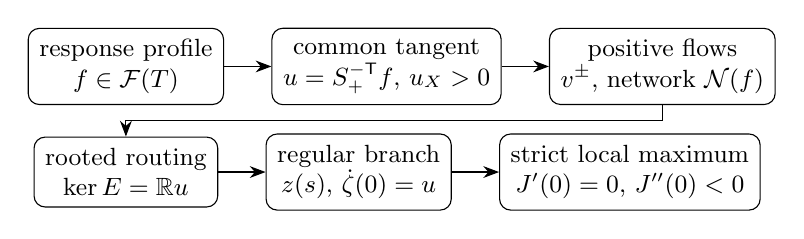
\begin{tikzpicture}[node distance=4mm and 6mm, every node/.style={draw, rounded corners, align=center, font=\small, inner sep=4pt}, >={Stealth[length=2mm]}]
\node (a) {response profile\\ $f\in\cone(T)$};
\node (b) [right=of a] {common tangent\\ $u=\Sp^{-\T}f$, $u_X>0$};
\node (c) [right=of b] {positive flows\\ $v^\pm$, network $\mathcal N(f)$};
\node (d) [below=of a] {rooted routing\\ $\Ker E=\R u$};
\node (e) [right=of d] {regular branch\\ $z(s)$, $\dot\zeta(0)=u$};
\node (f) [right=of e] {strict local maximum\\ $J'(0)=0$, $J''(0)<0$};
\draw[->] (a) -- (b); \draw[->] (b) -- (c); \draw[->] (c.south) -- ++(0,-2mm) -| (d.north);
\draw[->] (d) -- (e); \draw[->] (e) -- (f);
\end{tikzpicture}
\caption{The realization ladder of Section~\ref{sec:realizability}.  Each arrow is a theorem on the accessible rooted class; global optimality (Section~\ref{sec:global}) is a further, independent step.}
\label{fig:ladder}
\end{figure}

\subsection{The reconstructed network and the kinetic value set}
Fix complex matrices $(\Sp,\Sm)$ with $\Sp,S$ invertible, a controlled species $X$, the positive production mode $g$, integer weights $w\in\N^n$, and a current $J>0$.  Let $T=\Sp^{-1}\Sm$.

\begin{definition}[Normalized reconstruction]\label{def:reconstruction}
Let $f\in\cone(T)$ with $u:=\Sp^{-\T}f$ satisfying $u_X=1$, and let $q=q(f)$, $h=q\odot f=T^{\T}f$.  The \emph{reconstructed one-way flows} are
\begin{equation}\label{eq:flows}
v^-_i:=\frac{Jg_i}{q_i-1},\qquad v^+_i:=q_iv^-_i,
\end{equation}
and the \emph{reconstructed network} $\mathcal N(f)$ is the source with complexes $(\Sp,\Sm)$, controlled species $X$, and rate constants $k^\pm:=v^\pm$.
\end{definition}

\begin{lemma}[First-order realization]\label{lem:firstorder}
In the situation of Definition~\ref{def:reconstruction}: $v^\pm>0$; $v^+-v^-=Jg$; $v^+\odot f=v^-\odot h$; the unit state $z=\one$ is stationary for every noncontrolled species of $\mathcal N(f)$ with production current $J$; and if $\mathcal M$ is a smooth curve through $\one$ with logarithmic tangent $u$, then $\one$ is a zero-derivative optimum of $\mathcal N(f)$ in the forward regime with response profiles $(f,h)$ and $e^{A_w}=\Phi_w(f)$ there.
\end{lemma}

\begin{proof}
Positivity uses $J,g>0$ and $q>1$.  Next $v^+_i-v^-_i=(q_i-1)v^-_i=Jg_i$, and $v^+_if_i=q_if_iv^-_i=h_iv^-_i$.  At $z=\one$ every monomial equals $1$, so $j^\pm=v^\pm$ and $j=Jg$; hence $Sj=Je_X$, i.e.\ $S_Yj=0$ and $J(\one)=J$.  The last statement is Lemma~\ref{lem:response} read backwards: with tangent $u$ the response profiles are $\Sp^{\T}u=f$ and $\Sm^{\T}u=h$, and $v^+\odot f=v^-\odot h$ is the derivative balance.
\end{proof}

\begin{definition}[Regular strict-local realizability; kinetic capacity]\label{def:realizable}
Let $E$ be the Jacobian of the net current vector of $\mathcal N(f)$ with respect to $\zeta=\log z$ at $z=\one$.  We say that $f\in\cone(T)$ is \emph{regularly realizable} if $u=\Sp^{-\T}f$ has $u_X=1$ and
\begin{enumerate}[label=(\alph*)]
\item $\Ker E=\R u$;
\item there is $\lambda\in\R^n_{\ge0}\setminus\{0\}$ with $\lambda^{\T}E=0$ (necessarily $\lambda^{\T}g>0$);
\item the controlled reduced Jacobian is injective: if $w\in\R^n$ satisfies $w_X=0$ and $S_YEw=0$ then $w=0$.
\end{enumerate}
The \emph{strict-local kinetic value set} and \emph{capacity} are
\[
\Vloc=\{\Phi_w(f):\ f\in\cone(T),\ af\text{ regularly realizable for some }a>0\},\qquad \Kloc=\inf\Vloc ,
\]
with the convention $\inf\emptyset=0$.
\end{definition}

Propositions~\ref{prop:branch} and~\ref{prop:curvature} below show that conditions (a)--(c) guarantee an actual regular stationary branch of $\mathcal N(f)$ through $\one$ along which $J$ has a nondegenerate strict local maximum, so the name is justified.  The value set does not depend on $J$: replacing $J$ by $J'$ multiplies all rates by $J'/J$ and changes nothing else.

\begin{remark}[Physical meaning of $\Vloc$]\label{rem:physical}
Every source with complexes $(\Sp,\Sm)$, arbitrary positive rates, and a nondegenerate strict local maximum $z^*$ in the forward regime can be brought to the normalized form by the change of variables $z\mapsto z/z^*$, which multiplies each rate constant by a positive monomial in $z^*$ and does not change currents, ratios, response profiles or the nondegeneracy of the optimum.  Its rates then equal its one-way fluxes at the optimum, which by tight coupling and derivative balance are exactly~\eqref{eq:flows}.  Conversely every regularly realizable $f$ is realized by $\mathcal N(f)$.  Since $L\le\Phi_w(f)$ for the profile $f$ of any optimum in the forward regime (Theorem~\ref{thm:capacity}(ii)), Theorem~\ref{thm:main} implies that, on the accessible rooted class, $L(T,w)$ equals the infimum of $e^{NA^*_w}$ over all forward-regime zero-derivative optima of all sources with complexes $(\Sp,\Sm)$ and $X$ controlled, whether or not one restricts to nondegenerate optima.
\end{remark}

\subsection{The common tangent and control accessibility}
The first piece of information that the response matrix forgets is which coordinate is controlled.

\begin{lemma}[Control accessibility]\label{lem:access}
Let $f\in\cone(T)$ and $u=\Sp^{-\T}f$.  There is $a>0$ with $(au)_X=1$ if and only if $\chi_X(f):=u_X=(\Sp^{-\T}f)_X>0$.  If a forward-regime optimum of a source with complexes $(\Sp,\Sm)$ and controlled species $X$ has response profile $f$, then $\chi_X(f)>0$.
\end{lemma}

\begin{proof}
The first statement is immediate.  For the second, the tangent of the optimum satisfies $u_X=1$ by the choice of parameter $s=\log z_X$, and $f=\Sp^{\T}u$ determines $u$.
\end{proof}

Thus a profile with $\chi_X(f)\le0$ lies in the response relaxation but cannot be the response of any optimum with $X$ controlled: the relaxation is strictly loose at such points.  This is why the class in Theorem~\ref{thm:main} requires accessibility of the whole cone.

\subsection{Response Laplacian and response routing}
\begin{definition}\label{def:laplacian}
For $f\in\cone(T)$ with $q=q(f)$, the \emph{response Laplacian} and the \emph{response-routing matrix} are
\begin{equation}\label{eq:LP}
\mathcal L_f:=\Diag(q)-T^{\T},\qquad (P_f)_{ij}:=\frac{T_{ji}f_j}{q_if_i}=\frac{T_{ji}f_j}{(T^{\T}f)_i}.
\end{equation}
\end{definition}

\begin{lemma}[Structure of the response Laplacian]\label{lem:laplacian}
Let $f\in\cone(T)$.
\begin{enumerate}[label=(\roman*)]
\item $\mathcal L_ff=0$, and $P_f\one=\one$ (each row of $P_f$ sums to one).
\item $\mathcal L_f=\Diag(q\odot f)\,(I-P_f)\,\Diag(f)^{-1}$; consequently $\Ker\mathcal L_f=\Diag(f)\Ker(I-P_f)$.
\item If $T\ge0$ entrywise then $P_f\ge0$ is row-stochastic; its support digraph, with an edge $i\to j$ whenever $(P_f)_{ij}>0$, equals the digraph $G(T)$ with an edge $i\to j$ whenever $T_{ji}>0$, and does not depend on $f$.
\item (Current Jacobian.)  Let $E$ be as in Definition~\ref{def:realizable}.  Then
\begin{equation}\label{eq:Efactor}
E=\Diag(v^+)\Sp^{\T}-\Diag(v^-)\Sm^{\T}=\Diag(v^-)\,\mathcal L_f\,\Sp^{\T},
\end{equation}
so $\Ker E=\Sp^{-\T}\Ker\mathcal L_f$ and $\dim\Ker E=\dim\Ker(I-P_f)$.
\end{enumerate}
\end{lemma}

\begin{proof}
(i) $\mathcal L_ff=q\odot f-T^{\T}f=h-h=0$; $\sum_j(P_f)_{ij}=(T^{\T}f)_i/(q_if_i)=1$.  (ii) The $(i,j)$ entry of the right side is $q_if_i(\delta_{ij}-(P_f)_{ij})/f_j=q_i\delta_{ij}-T_{ji}$.  (iii) is clear from~\eqref{eq:LP} since $f>0$ and $q>0$.  (iv) Differentiating~\eqref{eq:massaction} at $\zeta=0$ for $\mathcal N(f)$ gives the first expression; then $\Diag(v^+)=\Diag(v^-)\Diag(q)$ and $\Sm^{\T}=T^{\T}\Sp^{\T}$.
\end{proof}

Lemma~\ref{lem:laplacian} is the central reduction: the neutral modes of the stationary problem at the reconstructed point are exactly the fixed vectors of the finite Markov chain $P_f$.  Note that $u=\Sp^{-\T}f\in\Ker E$ always, by (i) and (iv).

\subsection{Rooted routing: the sharp finite obstruction}
\begin{definition}\label{def:rooted}
A nonnegative matrix $P\in\R^{n\times n}$ \emph{has a common reachable state} if there is a state $r$ such that for every $i$ some power satisfies $(P^k)_{ir}>0$.  For a row-stochastic $P$ this says that $r$ is reachable from every state of the Markov chain with transition matrix $P$; equivalently, the chain has exactly one closed (terminal) communicating class.  Irreducible $P$ have this property.
\end{definition}

The equivalence in the definition is standard: a state reachable from all states lies in a closed class $C$, and no other closed class can reach $C$, so $C$ is the only closed class; conversely in a finite chain every state reaches some closed class, and if there is only one, every state reaches each of its members.  Only the ``common reachable state'' form is used in the proofs.

\begin{lemma}[Rooted maximum principle]\label{lem:maxprinciple}
Let $P\ge0$ be row-stochastic with a common reachable state.  Then every $v$ with $Pv=v$ is constant; that is, $\Ker(I-P)=\R\one$.
\end{lemma}

\begin{proof}
Let $M=\max_iv_i$ and $A=\{i:v_i=M\}$.  For $i\in A$, $M=v_i=\sum_jP_{ij}v_j\le M$ with equality only if $v_j=M$ whenever $P_{ij}>0$.  So $A$ is closed under transitions, and by induction $(P^k)_{ij}>0$ with $i\in A$ implies $j\in A$.  Since the common reachable state $r$ is reachable from any $i\in A$, $r\in A$, so $v_r=M$.  The same argument with the minimum gives $v_r=\min_iv_i$.  Hence $v$ is constant.
\end{proof}

\begin{lemma}[Nonnegative stationary vector]\label{lem:stationary}
Every row-stochastic $P\ge0$ has $\pi\in\R^n_{\ge0}\setminus\{0\}$ with $\pi^{\T}P=\pi^{\T}$.  If $P$ is irreducible, $\pi$ can be chosen strictly positive.
\end{lemma}

This is the Perron--Frobenius theorem for stochastic matrices, or equivalently the existence of a stationary distribution of a finite Markov chain~\cite{Sen06,KS76,BP94}.  (The formalization derives it from a fixed-point theorem, see Section~\ref{sec:formal}.)  A stationary distribution of a chain with one closed class is supported on that class and may vanish on transient states; this is why nonnegativity, not positivity, is the correct hypothesis in Proposition~\ref{prop:curvature}.

\begin{proposition}[Kernel and left null vector of the current Jacobian]\label{prop:kernel}
Let $T\ge0$, $f\in\cone(T)$, and suppose $P_f$ has a common reachable state.  Then $\Ker\mathcal L_f=\R f$ and $\Ker E=\R u$ with $u=\Sp^{-\T}f$.  Moreover there is $\lambda\in\R^n_{\ge0}\setminus\{0\}$ with $\lambda^{\T}E=0$, namely $\lambda_i=\pi_i/(q_if_iv^-_i)$ for a stationary vector $\pi$ of $P_f$; and $\lambda^{\T}g>0$.  If $P_f$ has $k\ge2$ closed classes, then $\dim\Ker E\ge2$.
\end{proposition}

\begin{proof}
Lemmas~\ref{lem:laplacian}(ii),(iv) and~\ref{lem:maxprinciple} give the kernels.  From $\pi^{\T}(I-P_f)=0$ and~\eqref{eq:LP}, $\mu^{\T}\mathcal L_f=0$ for $\mu_i=\pi_i/(q_if_i)$, and then $\lambda^{\T}E=\mu^{\T}\Diag(v^-)^{-1}\Diag(v^-)\mathcal L_f\Sp^{\T}=0$ for $\lambda_i=\mu_i/v^-_i$.  Positivity of $\lambda^{\T}g$ follows from $g>0$, $\lambda\ge0$, $\lambda\ne0$.  For the last claim, the indicator vector of each closed class is a fixed vector of $P_f$, and indicators of distinct classes are linearly independent.
\end{proof}

\subsection{The controlled reduced Jacobian and the branch}
The stationary equations of the noncontrolled species are $S_Yj(z)=0$, whose derivative at $\one$ is $S_YE$, not $E$ itself.  The control removes one direction.

\begin{proposition}[Regular branch]\label{prop:branch}
Assume $\Ker E=\R u$ with $u_X=1$ and that $\lambda\ge0$, $\lambda\ne0$, satisfies $\lambda^{\T}E=0$.  Then:
\begin{enumerate}[label=(\roman*)]
\item the controlled reduced Jacobian is injective: $w_X=0$ and $S_YEw=0$ imply $w=0$; equivalently the augmented linear map $w\mapsto(S_YEw,\,w_X)\in\R^{n-1}\times\R$ is invertible;
\item there is a smooth curve $s\mapsto z(s)\in\R^n_{>0}$ defined near $s=0$ with $z(0)=\one$, $\log z_X(s)=s$, $S_Yj(z(s))=0$, and logarithmic tangent $\dot\zeta(0)=u$; near $\one$ it is the whole stationary fiber $\mathcal M$ of $\mathcal N(f)$;
\item along this branch $J(s)=S_Xj(z(s))$ satisfies $J(0)=J$ and $J'(0)=0$.
\end{enumerate}
\end{proposition}

\begin{proof}
(i) Let $w_X=0$ and $S_YEw=0$.  Since $S$ is invertible and $S_Yg=0$, $\Ker S_Y=\R g$, so $Ew=cg$ for some $c$.  Then $0=\lambda^{\T}Ew=c\,\lambda^{\T}g$ and $\lambda^{\T}g>0$ give $c=0$.  So $w\in\Ker E=\R u$, $w=au$, and $0=w_X=au_X=a$.  Injectivity of a linear map $\R^n\to\R^n$ is invertibility.

(ii) Consider $\Psi(\zeta,s)=(S_Yj(e^\zeta),\ \zeta_X-s)$, smooth from $\R^n\times\R$ to $\R^n$, with $\Psi(0,0)=0$ by Lemma~\ref{lem:firstorder}.  Its derivative in $\zeta$ at $(0,0)$ is the augmented map of (i), which is invertible, so the inverse function theorem yields a smooth $\zeta(s)$ with $\Psi(\zeta(s),s)=0$, and every solution near $(0,0)$ is of this form.  Differentiating $S_Yj(e^{\zeta(s)})=0$ and $\zeta_X(s)=s$ at $0$ gives $S_YE\dot\zeta(0)=0$ and $\dot\zeta_X(0)=1$; since $u$ satisfies the same two conditions and the augmented map is injective, $\dot\zeta(0)=u$.

(iii) $J(0)=J$ by Lemma~\ref{lem:firstorder}; $\dot j(0)=E\dot\zeta(0)=Eu=0$, and $j=Jg$ along the branch gives $J'(0)g=0$.
\end{proof}

\subsection{Curvature: an exact left-null identity}
\begin{proposition}[Curvature identity]\label{prop:curvature}
In the situation of Proposition~\ref{prop:branch}, let $v=\ddot\zeta(0)$.  Then
\begin{equation}\label{eq:secondjet}
\ddot j(0)=Ev-J\,g\odot f\odot h,
\end{equation}
and consequently
\begin{equation}\label{eq:curvature}
J''(0)=-J\,\frac{\lambda^{\T}(g\odot f\odot h)}{\lambda^{\T}g}<0 .
\end{equation}
Hence $\one$ is a nondegenerate strict local maximum of the production current along the branch, and $f$ is regularly realizable in the sense of Definition~\ref{def:realizable}.  Writing $\mu_i=\lambda_ig_i/\lambda^{\T}g$, so that $\mu\ge0$ and $\sum_i\mu_i=1$,
\begin{equation}\label{eq:average}
-\frac{J''(0)}{J(0)}=\sum_i\mu_if_ih_i,\qquad\min_{\mu_i>0}f_ih_i\le-\frac{J''(0)}{J(0)}\le\max_{\mu_i>0}f_ih_i .
\end{equation}
\end{proposition}

\begin{proof}
From~\eqref{eq:massaction}, $j^\pm_\rho(s)=v^\pm_\rho\exp((S_\pm^{\T}\zeta(s))_\rho)$, so
\[
\ddot j^\pm_\rho(0)=v^\pm_\rho\big[(S_\pm^{\T}u)_\rho^2+(S_\pm^{\T}v)_\rho\big],
\]
and $\ddot j(0)=Ev+v^+\odot f^{\odot2}-v^-\odot h^{\odot2}$.  Using $v^+=q\odot v^-$, $h=q\odot f$ and $v^-\odot(q-\one)=Jg$,
\[
v^+\odot f^{\odot2}-v^-\odot h^{\odot2}=v^-\odot(q-q^{\odot2})\odot f^{\odot2}=-v^-\odot(q-\one)\odot f\odot h=-J\,g\odot f\odot h .
\]
Since $j=Jg$ along the branch, $\ddot j(0)=J''(0)g$.  Pairing with $\lambda$ kills $Ev$ and gives $J''(0)\lambda^{\T}g=-J\lambda^{\T}(g\odot f\odot h)$.  The right side of~\eqref{eq:curvature} is negative because $J>0$, $\lambda\ge0$, $\lambda\neq0$ and $g,f,h>0$.  A smooth function with $J'(0)=0$ and $J''(0)<0$ has a strict local maximum at $0$.  The average form is a rewriting, and the bounds follow because $\mu$ is a probability vector.
\end{proof}

The identity~\eqref{eq:average} explains why negative curvature is robust rather than a delicate cancellation: once the branch exists, the normalized curvature is an average of the positive response products $f_ih_i$ over the recurrent routing support, weighted by the stationary distribution of the routing chain.  In the irreducible case all weights are positive; in the rooted case transient coordinates may carry zero weight.

\subsection{The accessible rooted class and the capacity theorem}
\begin{definition}[Accessible rooted sources]\label{def:class}
A source with complexes $(\Sp,\Sm)$, controlled species $X$ and response matrix $T=\Sp^{-1}\Sm$ is \emph{accessible and rooted} if
\begin{enumerate}[label=(\roman*)]
\item $T\ge0$ entrywise;
\item the digraph $G(T)$ (edge $i\to j$ whenever $T_{ji}>0$) has a vertex reachable from every vertex, equivalently a unique terminal strong component;
\item every $f\in\cone(T)$ satisfies $\chi_X(f)=(\Sp^{-\T}f)_X>0$.
\end{enumerate}
It is \emph{accessible and irreducible} if (i), (iii) hold and $G(T)$ is strongly connected.
\end{definition}

By Lemma~\ref{lem:laplacian}(iii), conditions (i)--(ii) say exactly that for every $f\in\cone(T)$ the routing matrix $P_f$ is nonnegative and has a common reachable state; this is the form in which the class is formalized (Section~\ref{sec:formal}).  Accessible irreducible sources are accessible and rooted.  Condition (iii) is automatic when the $X$-th column of $\Sp^{-1}$ is nonnegative and nonzero, since $\chi_X(f)=\sum_\rho(\Sp^{-1})_{\rho X}f_\rho$; this is the case when $\Sp$ is diagonal, as in all examples of Sections~\ref{sec:counterexample}--\ref{sec:capacity}.

\begin{theorem}[Kinetic exactness of the response capacity]\label{thm:main}
Let the source be accessible and rooted, with positive production mode $g$, integer weights $w\in\N^n$, and $J>0$.  Then every $f\in\cone(T)$ has a positive multiple that is regularly realizable, so
\[
\Vresp(T,w)=\Vloc\qquad\text{and}\qquad L(T,w)=\Kloc .
\]
In words: for every response profile in the forward-response cone there is a positive mass-action network with complexes $(\Sp,\Sm)$ and controlled species $X$ that has a regular stationary branch through a state with response profile $f$, along which the production current has a nondegenerate strict local maximum with $e^{NA^*_w}=\Phi_w(f)$.
\end{theorem}

\begin{proof}
The inclusion $\Vloc\subseteq\Vresp$ holds by definition (a regularly realizable profile lies in the cone, and $\Phi_w$ is scale invariant).  Conversely let $f\in\cone(T)$.  By (iii) and Lemma~\ref{lem:access}, replacing $f$ by $f/\chi_X(f)$ we may assume $u_X=1$, without changing $\Phi_w(f)$ or membership in the cone.  Form $\mathcal N(f)$ (Definition~\ref{def:reconstruction}).  By (i)--(ii) and Lemma~\ref{lem:laplacian}(iii), $P_f$ is nonnegative, row-stochastic and has a common reachable state, so Proposition~\ref{prop:kernel} gives $\Ker E=\R u$ and a left null vector $\lambda\ge0$, $\lambda\neq0$, with $\lambda^{\T}g>0$.  Proposition~\ref{prop:branch}(i) gives condition (c) of Definition~\ref{def:realizable}, and (a), (b) are what was just shown.  Hence $f$ is regularly realizable and $\Phi_w(f)\in\Vloc$.  The remaining assertions are Propositions~\ref{prop:branch} and~\ref{prop:curvature} and Lemma~\ref{lem:firstorder}.  Equality of the infima follows from equality of the sets (both empty if the cone is empty).
\end{proof}

\begin{corollary}[Irreducible case]\label{cor:irreducible}
For accessible irreducible sources the same conclusions hold, with a strictly positive left null vector $\lambda$ and strictly positive curvature weights $\mu$.
\end{corollary}

\begin{remark}[Why the rooted condition is the right one]\label{rem:sharp}
If $G(T)$ has $k\ge2$ terminal strong components, Proposition~\ref{prop:kernel} gives $\dim\Ker E\ge2$ for every $f\in\cone(T)$.  The single control constraint $w_X=0$ removes at most one direction, so the augmented derivative of Proposition~\ref{prop:branch}(i) is singular and the branch construction of this section fails for every profile.  Thus multiplicity of terminal classes is exactly the obstruction to the mechanism used here, and the passage from irreducibility (used in a first version of this work) to the rooted condition replaces a convenient sufficient hypothesis by the finite condition the argument actually needs.  We do not claim that $\Vresp=\Vloc$ fails for every source outside the class.
\end{remark}

\begin{example}[A rooted, non-irreducible source]\label{ex:rooted}
The source $\mathcal P_2$ of Section~\ref{sec:global}, $2X+3Y\rightleftharpoons2X+2Y$, $X+Y\rightleftharpoons2X+2Y$ with $X$ controlled, has $\Sp=\begin{pmatrix}2&1\\3&1\end{pmatrix}$, $\Sm=\begin{pmatrix}2&2\\2&2\end{pmatrix}$ and $T=\begin{pmatrix}0&0\\2&2\end{pmatrix}$.  Its routing digraph has edges $1\to2$ and $2\to2$ only: state $2$ is reachable from both states, but $1$ is not reachable from $2$, so $P_f$ is reducible with a transient state.  The cone is $\{f_1<2f_2\}$ (since $h=(2f_2,2f_2)$), and $\chi_X(f)=-f_1+3f_2>f_2>0$ on it.  Theorem~\ref{thm:main} applies while Corollary~\ref{cor:irreducible} does not.
\end{example}

\begin{remark}[Behaviour at the boundary of the cone]\label{rem:gauge}
The reconstruction~\eqref{eq:flows} appears to diverge as some $q_i\downarrow1$.  This is a gauge artifact: the response profile is a ray and the current $J$ is a free scale.  Choosing the representative with $J=\varepsilon$ and $q_i=1+\varepsilon r_i$ for fixed $r>0$ gives $v^-_i=g_i/r_i$, independent of $\varepsilon$, and $v^+_i=(1+\varepsilon r_i)g_i/r_i\to g_i/r_i$ as $\varepsilon\to0$.  So the physical one-way flows of the realizing networks remain bounded along profile sequences approaching the boundary $q\to\one$ where $\Phi_w\to1$.  This observation is not used in the proof of Theorem~\ref{thm:main}.
\end{remark}

\section{Response optimality as matrix balancing}\label{sec:scaling}

The response objective has a variational structure that connects the optimal-affinity problem with classical matrix scaling~\cite{Sin64,SK67,Idel16}.  Write $f_i=e^{s_i}$ and, for real weights $g\in\R^n$,
\begin{equation}\label{eq:logobjective}
F_g(s)=\sum_ig_i\Big[\log\Big(\sum_jT_{ji}e^{s_j}\Big)-s_i\Big]=\sum_ig_i\log q_i(f),
\end{equation}
so that $\log\Phi_w=F_w$.  This is the concave objective of~\cite[Supplementary Note~11]{DDL24}.

\begin{proposition}[Gradient is the routing residual]\label{prop:kkt}
Let $T\ge0$ have no zero column, $f>0$, $h=T^{\T}f>0$, $q=h/f$ and $P=P_f$ as in~\eqref{eq:LP}.  Then
\[
\nabla_sF_g=P^{\T}g-g .
\]
In particular an interior critical point of $F_g$, hence any interior local minimizer of $\Phi_w$ on $\cone(T)$ (with $g=w$), satisfies $P_f^{\T}w=w$: the production weights are stationary for the response-routing chain.
\end{proposition}

\begin{proof}
$\partial_{s_k}\sum_ig_i\log h_i=\sum_ig_iT_{ki}f_k/h_i=\sum_ig_iP_{ik}=(P^{\T}g)_k$, and $\partial_{s_k}\sum_ig_is_i=g_k$.
\end{proof}

\begin{proposition}[Attained matrix-scaling identity]\label{prop:dual}
Let $T>0$ entrywise, $f>0$, $h=T^{\T}f$, $P=P_f$, and suppose $P^{\T}g=g$ for some $g\in\R^n$.  Then the nonnegative matrix $M_{ij}=g_iP_{ij}$ has both marginals equal to $g$, $M\one=g=M^{\T}\one$, and
\begin{equation}\label{eq:entropy}
\sum_{i,j}g_iP_{ij}\log\frac{T_{ji}}{P_{ij}}=F_g(s).
\end{equation}
\end{proposition}

\begin{proof}
$M\one=g$ by row-stochasticity and $M^{\T}\one=P^{\T}g=g$.  Since $T_{ji}/P_{ij}=h_i/f_j$, the left side of~\eqref{eq:entropy} is $\sum_ig_i\log h_i\sum_jP_{ij}-\sum_j\log f_j\sum_ig_iP_{ij}=\sum_ig_i\log h_i-\sum_jg_j\log f_j$.
\end{proof}

The matrix $M=\Diag(g)P_f=\Diag(g/h)\,T^{\T}\Diag(f)$ is a diagonal scaling of $T^{\T}$ with prescribed row and column sums $g$, and~\eqref{eq:entropy} is the Gibbs variational identity for the log-sum-exp terms in~\eqref{eq:logobjective}.  The scaling theory itself is classical (Sinkhorn~\cite{Sin64}, Sinkhorn--Knopp~\cite{SK67}; see~\cite{Idel16} for a survey); what is specific to the present setting is the identification of the scaled matrix with the infinitesimal response routing of an autocatalytic source, of the prescribed marginal with the production mode, of the balance condition with the first-order condition for optimal affinity, and, through Theorem~\ref{thm:main}, of the balanced profile with a genuine strict local mass-action optimum.  Existence, uniqueness modulo scale, and algorithms for such balancing states under support conditions on $T$ can be imported from that theory; we do not pursue this here.

\section{Global optimality is a separate layer}\label{sec:global}

Theorem~\ref{thm:main} concerns the jet of one branch.  A unique global maximum is a statement about the whole positive stationary fiber $\mathcal M$ and requires additional source-level information.  We record the exact form this information takes and give one reusable mechanism that produces it.

\begin{remark}[Global certificates]\label{rem:certificate}
Let $f$ be regularly realizable for a source and $\mathcal N=\mathcal N(f)$ with fiber $\mathcal M$ and current $J(\cdot)$ on $\mathcal M$.  Then $\one$ is a unique global maximum of $J$ on $\mathcal M$ if and only if the pair of conditions ``$J(z)\le J$ for all $z\in\mathcal M$'' and ``$J(z)=J$, $z\in\mathcal M$ imply $z=\one$'' holds.  This is a tautology, but a useful one: it isolates the datum (a nonnegative gap on the fiber with a unique zero) that response data do not contain.  We make no claim that this datum is a function of $(T,w,f)$ alone.  A bounded exact search over $7{,}332$ small integer sources during this work found $800$ pairs with identical response data and no pair differing in global behaviour, but a finite search is not evidence of a theorem, and the two families below were found by algebra, not by search.
\end{remark}

\subsection{The tangent-gap certificate}
\begin{theorem}[Tangent gap]\label{thm:tangentgap}
Let $\phi\colon\R_{>0}\to\R_{>0}$ with $\phi(1)=1$, let $a\in\R$, and suppose $1+a(y-1)\le\phi(y)$ for all $y>0$ with equality only at $y=1$.  Then
\[
\mathcal J(y):=\frac{1+a(y-1)}{\phi(y)}\le1\quad(y>0),\qquad\text{with equality if and only if }y=1 .
\]
\end{theorem}

\begin{proof}
Divide the hypothesis by $\phi(y)>0$.
\end{proof}

The theorem is trivial; its content is the observation that both global families in this paper have this form after elimination of the fiber: the reduced current is a normalized tangent line divided by a positive denominator that lies above its tangent, and the factorized gaps~\eqref{eq:H1} and~\eqref{eq:powergap} are the certificates that the inequality is strict away from the optimum.  For $\phi$ strictly convex and differentiable with $a=\phi'(1)$ the hypothesis is automatic.

\subsection{An infinite two-reaction family with unique global maxima}
\begin{definition}[The power family $\mathcal P_d$]\label{def:power}
For an integer $d\ge2$ let $(c,e)=(d/2,1)$ if $d$ is even and $(c,e)=((d+1)/2,2)$ if $d$ is odd, so that $2c-e+1=d$.  Let $\mathcal P_d$ be the source with $X$ controlled and reactions
\[
R_1:\ (c+1)X+(e+2)Y\rightleftharpoons(c+1)X+(e+1)Y,\qquad R_2:\ cX+eY\rightleftharpoons(c+1)X+(e+1)Y,
\]
both with rate constants $(k^+,k^-)=(d,d-1)$.  Thus
\[
\Sp=\begin{pmatrix}c+1&c\\e+2&e\end{pmatrix},\qquad\Sm=\begin{pmatrix}c+1&c+1\\e+1&e+1\end{pmatrix},\qquad S=\begin{pmatrix}0&1\\-1&1\end{pmatrix},
\]
with $\det\Sp=e-2c=1-d$, $\det S=1$, and $g=w=\one$.
\end{definition}

For $d=4$ this is the source $\Sp=\begin{pmatrix}3&2\\3&1\end{pmatrix}$, $\Sm=\begin{pmatrix}3&3\\2&2\end{pmatrix}$ with rates $(4,3)$, $(4,3)$, which was found by an exact enumeration of small integer sources; the family was then read off from its elimination.

\begin{theorem}[Power family]\label{thm:power}
For every integer $d\ge2$ the source $\mathcal P_d$ has stationary fiber $\mathcal M=\{(x,y)>0:\ xy^2=1\}$, on which the production current is
\begin{equation}\label{eq:powercurrent}
J_d(y)=\frac{dy-(d-1)}{y^d},
\end{equation}
and
\begin{equation}\label{eq:powergap}
1-J_d(y)=\frac{(y-1)^2W_d(y)}{y^d},\qquad W_d(y)=\sum_{k=0}^{d-2}(d-1-k)\,y^k>0\quad(y>0).
\end{equation}
Hence the unit state is the unique global maximum of $J$ on $\mathcal M$, with $J=1$, and the optimal affinity there is
\[
e^{A^*}=\Big(\frac d{d-1}\Big)^2,\qquad q_1=q_2=\frac d{d-1}.
\]
The family is accessible and rooted for every $d$, and irreducible for $d\ge4$.
\end{theorem}

\begin{proof}
The currents are $j_1=x^{c+1}y^{e+1}\big(dy-(d-1)\big)$ and $j_2=x^cy^e\big(d-(d-1)xy\big)$.  The $Y$-row of $S$ is $(-1,1)$, so stationarity of $Y$ is $j_1=j_2$; dividing by $x^cy^e>0$ this reads $xy\,(dy-(d-1))=d-(d-1)xy$, i.e.\ $d\,xy^2=d$, so $\mathcal M=\{xy^2=1\}$.  The $X$-row is $(0,1)$, so $J=j_2$, and on $\mathcal M$, with $x=y^{-2}$, $J=y^{e-2c}\big(d-(d-1)y^{-1}\big)=(dy-(d-1))/y^{2c-e+1}$, which is~\eqref{eq:powercurrent}.  Next, $y^d-dy+d-1=(y^d-1)-d(y-1)=(y-1)\sum_{k=0}^{d-1}(y^k-1)=(y-1)^2\sum_{k=1}^{d-1}\sum_{m=0}^{k-1}y^m$, which is~\eqref{eq:powergap}; $W_d>0$ for $y>0$ since $d\ge2$.  Theorem~\ref{thm:tangentgap} with $\phi(y)=y^d$ and $a=d$ (or directly~\eqref{eq:powergap}) gives $J_d\le1$ with equality only at $y=1$, i.e.\ at $(x,y)=(1,1)$.  At the unit state both reactions have $j^+=d$, $j^-=d-1$, so $q_1=q_2=d/(d-1)$ and $e^{A^*}=(d/(d-1))^2$ since $g=(1,1)$.  Finally $T=\Sp^{-1}\Sm$ has $\Sm$ with both columns equal to $(c+1,e+1)^{\T}$, so both columns of $T$ equal $\Sp^{-1}(c+1,e+1)^{\T}=\frac1{1-d}\big(e(c+1)-c(e+1),\ -(e+2)(c+1)+(c+1)(e+1)\big)^{\T}=\frac1{d-1}\big(c-e,\ c+1\big)^{\T}$; both entries are nonnegative, the second is positive, and the first is positive iff $c>e$, i.e.\ $d\ge4$.  Thus the routing digraph has edges from both states into state $2$, and also into state $1$ when $d\ge4$; so it is rooted, and strongly connected iff $d\ge4$.  For accessibility, write $\tau=\frac{(c-e)f_1+(c+1)f_2}{d-1}$, so that $h=T^{\T}f=\tau\one$.  The cone condition $q_1=\tau/f_1>1$ reads $(c+1)f_2>(d-1-c+e)f_1=c\,f_1$, using $d-1=2c-e$.  Since $\Sp^{-1}=\frac1{1-d}\begin{pmatrix}e&-c\\-(e+2)&c+1\end{pmatrix}$,
\[
\chi_X(f)=(\Sp^{-\T}f)_X=\frac{(e+2)f_2-e\,f_1}{d-1}>\frac{\big(e+2-e\tfrac{c+1}{c}\big)f_2}{d-1}=\frac{(2-e/c)\,f_2}{d-1}>0,
\]
because $e/c\le1$ in both parities ($e=1\le c$, or $e=2\le c$).
\end{proof}

\begin{remark}
For the power family the gross ratio is $\beta/\alpha=(2c+2)/(2c+1)$ and $(d/(d-1))^2>\beta/\alpha$, so the family is consistent with Conjecture~\ref{conj:gross}; its role is to show that exact global statements are available for an infinite class through the tangent-gap mechanism.  Because each member has a unique global maximum realizing the affinity $(d/(d-1))^2$, the global and strict-local affinity value sets indexed by the family coincide.  The recycling family of Theorem~\ref{thm:family} is a second, independent instance of the same mechanism, with $\phi(y)$ read off from~\eqref{eq:H1}.
\end{remark}

\section{Interacting cores: compatibility layers that do not collapse}\label{sec:cores}

The realizability ladder of Section~\ref{sec:realizability} concerns a single square source.  Networks with several overlapping autocatalytic cores raise a prior question: can the cores run simultaneously in their productive directions at all?  Kosc, Kuperberg, Rajon and Charlat~\cite{KKRC25} showed that thermodynamic consistency of the kinetics constrains which cores are jointly realizable.  We isolate three layers of ``joint realizability'' and show by exact examples that they are strictly ordered, so that the local theory of Section~\ref{sec:realizability} cannot be glued across cores by a single compatibility descriptor.

\begin{definition}[Compatibility layers]\label{def:layers}
Let $\mathcal Q$ be a reversible network with species set $\mathcal S$, reactions $\mathcal R$, reactant and product complexes $\rho(r),\pi(r)\in\N^{\mathcal S}$, and \emph{barrier} kinetics: for $z\in\R^{\mathcal S}_{>0}$ the current of $r$ is $c_r(z)=b_r\big(z^{\rho(r)}-z^{\pi(r)}\big)$ with $b_r>0$, where $z^{\kappa}=\prod_sz_s^{\kappa_s}$.  (This is mass action with all equilibrium constants equal to one, a convenient thermodynamically consistent normalization.)  A \emph{motif} is a pair $C=(\mathcal S_C,\mathcal R_C)$ of nonempty subsets; it is \emph{productive} for a current vector $v\in\R^{\mathcal R}$ if $\sum_{r\in\mathcal R_C}\big(\pi(r)_s-\rho(r)_s\big)v_r>0$ for every $s\in\mathcal S_C$.  A \emph{core family} is a finite collection of motifs, each a minimal productive motif (a primitive autocatalytic core in the sense of~\cite[Definitions~1--2]{KKRC25}), together with an orientation $\epsilon_r\in\{\pm1\}$ of every reaction.  The family is
\begin{enumerate}[label=(\roman*)]
\item \emph{direction compatible} if there is a potential $\mu\in\R^{\mathcal S}$ with $\epsilon_r\sum_s\big(\rho(r)_s-\pi(r)_s\big)\mu_s>0$ for every $r$;
\item \emph{stoichiometrically compatible} (multi-PAC) if there is $v$ with $\epsilon_rv_r>0$ for all $r$ such that every core is productive for $v$;
\item \emph{complex-level compatible} if there is a positive activity $y_\kappa>0$ for every complex $\kappa$ occurring in $\mathcal Q$ such that, with $\tilde c_r=b_r(y_{\rho(r)}-y_{\pi(r)})$, $\epsilon_r\tilde c_r>0$ for all $r$ and every core is productive for $\tilde c$;
\item \emph{kinetically compatible} (multi-CAC) if there is $z\in\R^{\mathcal S}_{>0}$ with $\epsilon_rc_r(z)>0$ for all $r$ and every core productive for $c(z)$.
\end{enumerate}
\end{definition}

Kinetic compatibility implies complex-level compatibility (take $y_\kappa=z^\kappa$) and direction compatibility (take $\mu=\log z$); complex-level compatibility drops the requirement that complex activities be monomials in one species vector.  Neither implication reverses.

\begin{theorem}[Direction compatibility does not imply complex-level compatibility]\label{thm:magnitude}
Let $\mathcal Q$ have species $A,B,C,D$, reactions $r_0\colon A\rightleftharpoons B$, $r_1\colon B\rightleftharpoons C$, $r_2\colon C\rightleftharpoons2A$, $r_3\colon B\rightleftharpoons D$, $r_4\colon D\rightleftharpoons2A$, barriers $(1,1,1,10,10)$, orientations all $+1$, and the two cores $C_{\mathrm L}=(\{A,B,C\},\{r_0,r_1,r_2\})$, $C_{\mathrm R}=(\{A,B,D\},\{r_0,r_3,r_4\})$.  This family is stoichiometrically compatible and direction compatible but not complex-level compatible, hence not kinetically compatible.
\end{theorem}

\begin{proof}
Stoichiometric compatibility: $v=(1,\tfrac45,\tfrac35,\tfrac45,\tfrac35)$ gives net productions $A\colon-1+\tfrac65$, $B\colon1-\tfrac45$, $C\colon\tfrac45-\tfrac35$ in $C_{\mathrm L}$ and the same numbers with $D$ in $C_{\mathrm R}$, all positive.  Direction compatibility: $\mu=(-1,-\tfrac32,-\tfrac95,-\tfrac95)$ gives $\mu_A-\mu_B=\tfrac12$, $\mu_B-\mu_C=\tfrac3{10}$, $\mu_C-2\mu_A=\tfrac15$, $\mu_B-\mu_D=\tfrac3{10}$, $\mu_D-2\mu_A=\tfrac15$.  Suppose complex activities $y_A,y_B,y_C,y_D,y_{2A}>0$ realize the family with currents $\tilde c_0=y_A-y_B$, $\tilde c_1=y_B-y_C$, $\tilde c_2=y_C-y_{2A}$, $\tilde c_3=10(y_B-y_D)$, $\tilde c_4=10(y_D-y_{2A})$, all positive.  Productivity of $C_{\mathrm L}$ at $A$, $B$, $C$ reads $2\tilde c_2>\tilde c_0$, $\tilde c_0>\tilde c_1$, $\tilde c_1>\tilde c_2$, so $\tilde c_0<\tilde c_1+\tilde c_2<2\tilde c_0$; productivity of $C_{\mathrm R}$ likewise gives $\tilde c_0<\tilde c_3+\tilde c_4<2\tilde c_0$.  But $\tilde c_1+\tilde c_2=y_B-y_{2A}$ and $\tilde c_3+\tilde c_4=10(y_B-y_{2A})$, so $10(\tilde c_1+\tilde c_2)<2\tilde c_0<2(\tilde c_1+\tilde c_2)$, impossible since $\tilde c_1+\tilde c_2>0$.
\end{proof}

\begin{theorem}[Complex-level compatibility does not imply kinetic compatibility]\label{thm:toric}
Let $\mathcal Q$ have species $A,B$, reactions $r_0\colon A\rightleftharpoons B$, $r_1\colon B\rightleftharpoons2A$, $r_2\colon B\rightleftharpoons3A$, barriers $(1,1,2)$, orientations $+1$, and cores $C_{\mathrm L}=(\{A,B\},\{r_0,r_1\})$, $C_{\mathrm R}=(\{A,B\},\{r_0,r_2\})$.  This family is stoichiometrically, direction and complex-level compatible but not kinetically compatible.
\end{theorem}

\begin{proof}
Stoichiometric: $v=(1,\tfrac34,\tfrac12)$ gives $A\colon-1+\tfrac32$, $B\colon1-\tfrac34$ in $C_{\mathrm L}$ and $A\colon-1+\tfrac32$, $B\colon1-\tfrac12$ in $C_{\mathrm R}$.  Direction: $\mu=(-1,-\tfrac32)$ gives $\mu_A-\mu_B=\tfrac12$, $\mu_B-2\mu_A=\tfrac12$, $\mu_B-3\mu_A=\tfrac32$.  Complex-level: $y_A=4$, $y_B=3$, $y_{2A}=\tfrac94$, $y_{3A}=\tfrac{11}4$ give $\tilde c=(1,\tfrac34,\tfrac12)=v$.  Kinetic: suppose $z=(a,b)>0$ with $c_0=a-b>0$, $c_1=b-a^2>0$, $c_2=2(b-a^3)>0$, and both cores productive: $2c_1>c_0>c_1$ and $3c_2>c_0>c_2$.  From $a>b>a^2$ we get $a<1$.  The inequality $c_1>c_0/2$ reads $3b>a+2a^2$, and $c_0>c_2$ reads $3b<a+2a^3$; together $a^2<a^3$, i.e.\ $a>1$, a contradiction.
\end{proof}

In the first example the shared complex $2A$ couples the two private branches through their barriers; in the second, the complexes $A$, $2A$, $3A$ can be assigned independent activities but not consistent powers of a single concentration.  For the optimal-affinity problem the lesson is that a module of an interacting network cannot be summarized by its productive direction, or even by its complex-level current magnitudes, when one asks whether a common positive kinetic state realizes all modules at once; the typed layers of Definition~\ref{def:layers} must be carried separately, exactly as the response, branch, curvature and global layers of Sections~\ref{sec:realizability}--\ref{sec:global} are separate for a single source.

\section{Formal verification}\label{sec:formal}

All theorems of Sections~\ref{sec:counterexample}--\ref{sec:cores} were developed together with a formalization in Lean~4 (toolchain \texttt{leanprover/lean4:v4.30.0}) against a frozen Mathlib manifest, compiled with warnings treated as errors, and checked to use no \texttt{sorry} and no axioms beyond \texttt{propext}, \texttt{Classical.choice} and \texttt{Quot.sound}.  The development is organized in three libraries corresponding to Sections~\ref{sec:counterexample}, \ref{sec:capacity} and \ref{sec:realizability}--\ref{sec:cores}; each has a root declaration (the second library has two) whose type is the conjunction of the results claimed.  Table~\ref{tab:receipts} lists the roots and the SHA-256 hashes of the root source files at verification time.  Appendix~\ref{app:lean} maps the numbered statements of this paper to declarations.

\begin{table}[H]
\centering\small
\begin{tabular}{@{}>{\raggedright\arraybackslash}p{0.34\textwidth}>{\raggedright\arraybackslash}p{0.36\textwidth}l@{}}
\toprule
Library and root file & Root declaration & Source SHA-256 (prefix) \\
\midrule
\texttt{OptimalAffinity/\allowbreak Main.lean} & \texttt{optimalAffinity\_\allowbreak \allowbreak seedLowerBound\_\allowbreak false} & \texttt{47ebd9ed ce9fbd22} \\
\texttt{OptimalAffinityCorrected/\allowbreak Main.lean} & \texttt{correctedTheoryClosure} & \texttt{e51ef928 df1b2841} \\
\texttt{OptimalAffinityCorrected/\allowbreak SourceClosure.lean} & \texttt{sourceClosurePackage} & \texttt{0159dd95 7b7873a9} \\
\texttt{OptimalAffinityRealizability/\allowbreak Main.lean} & \texttt{optimalAffinityKinetic\allowbreak Realizability\allowbreak PublicationResolution} & \texttt{39d78259 ed36431b} \\
\bottomrule
\end{tabular}
\caption{Root declarations and receipts.  All receipts record Lean 4.30.0, the same Mathlib manifest (SHA-256 prefix \texttt{a8df0b60}), exit code $0$, empty error output, warnings as errors, and the three standard axioms.}
\label{tab:receipts}
\end{table}

\subsection{The three roots}
The refutation library formalizes the two-species two-reaction network as a record with separate reactant and product stoichiometries and real rate constants, the predicate \texttt{SourceValid} (positive rates, invertible net stoichiometry, unit production mode, $0<\alpha<\beta$, conservation of $Y$ in the overall reaction, existence of a detailed-balance state), the predicate \texttt{IsUniqueGlobalMaximum}, and the two-by-two instance of Conjecture~\ref{conj:gross}:
\begin{lstlisting}
def TwoByTwoSeedLowerBound : Prop :=
  ∀ (N : Network) (x y : ℝ),
    SourceValid N → IsUniqueGlobalMaximum N x y →
    seedRatio N ≤ affinityExp N x y

theorem oa2x2_sourceFaithfulCounterexample :
    ∃ (N : Network) (x y : ℝ),
      SourceValid N ∧ IsUniqueGlobalMaximum N x y ∧ affinityExp N x y < seedRatio N

theorem optimalAffinity_seedLowerBound_false : ¬ TwoByTwoSeedLowerBound
\end{lstlisting}
The global-maximum proof is the polynomial identity~\eqref{eq:oa2x2cert}, discharged by \texttt{ring}.

The corrected-theory library defines \texttt{ForwardResponse}, \texttt{responseObjective}, \texttt{responseValueSet} and \texttt{response\allowbreak Profile\allowbreak Bound} (Definition~\ref{def:capacity}, with natural-number weights) and proves \texttt{responseProfileBound\_\allowbreak isGLB}, \texttt{responseProfileBound\_\allowbreak applies\_\allowbreak at\_\allowbreak optimum} and \texttt{grossBound\_\allowbreak holdsOnResponseCone\_\allowbreak iff} (Theorem~\ref{thm:capacity}); the recycling family with its literal currents, the identities~\eqref{eq:H1}--\eqref{eq:HJ} (\texttt{family\_\allowbreak H1\_\allowbreak certificate}, \texttt{family\_\allowbreak HJ\_\allowbreak gap}), \texttt{family\_\allowbreak uniqueGlobalMaximum} for every natural $m\ge2$ and every real $1<r<2$, and \texttt{noUniformPositiveSourceAffinityGap} (Theorem~\ref{thm:family}, Corollary~\ref{cor:nogap}); and the zero-diagonal circuit with \texttt{zeroDiagonalSourceCounterexample} (Theorem~\ref{thm:zerodiag}).  Its two roots bundle these statements.

The realizability library works with a record \texttt{SquareSource} (real nonnegative complex matrices, positive rates, a controlled index, and invertibility of $\Sp$ and $S$ as \texttt{IsUnit} of determinants) and the predicate \texttt{ControlledProductionMode} ($Sg=e_X$).  Its publication root is
\begin{lstlisting}
theorem optimalAffinityKineticRealizabilityPublicationResolution :
    SharpLiteralLocalCapacityResolution ∧
      PowerFamilyGlobalResolution ∧
      InteractingCoreBoundaryResolution
\end{lstlisting}
where the first conjunct is Theorem~\ref{thm:main} in the form
\begin{lstlisting}
theorem rawSquareSource_sharpCapacityEquality {n : ℕ} [Nonempty (Fin n)]
    (source : SquareSource n) (weights : Fin n → ℕ)
    (J : ℝ) (production : Fin n → ℝ)
    (hclass : AccessibleRootedResponseClass source)
    (hJ : 0 < J) (hproduction : ∀ i, 0 < production i)
    (hmode : ControlledProductionMode source production) :
    responseLayerCapacity (responseMatrix source) weights =
      strictLocalCapacity source weights J production
\end{lstlisting}
Here \texttt{Accessible\allowbreak Rooted\allowbreak Response\allowbreak Class} requires, for every \texttt{f} in the cone, \texttt{ControlAccessible} ($\chi_X(f)>0$), nonnegativity of the routing matrix, and \texttt{HasCommon\allowbreak Reachable\allowbreak State} of the routing matrix (Definition~\ref{def:rooted}); \texttt{strictLocalCapacity} is the infimum of the objective over profiles admitting a \texttt{StrictLocal\allowbreak Realization\allowbreak Witness}, a record containing $q,h,u,\lambda$ and a certificate consisting of the first-order realization of Lemma~\ref{lem:firstorder}, the kernel statements $\Ker\mathcal L_f=\R f$ and $\Ker E=\R u$, the left null vector $\lambda\ge0$ with $\lambda^{\T}g\neq0$, the injectivity of the controlled reduced Jacobian, and $u_X=1$ (Definition~\ref{def:realizable}).  The equality is proved as an equality of value sets and then pushed through the infimum, so it holds without any nonemptiness hypothesis.  Separately compiled are the actual branch and strict maximum (Propositions~\ref{prop:branch} and~\ref{prop:curvature}: \texttt{exists\_\allowbreak localPositiveLogBranch} via Mathlib's inverse function theorem, \texttt{smoothLocalBranch\_\allowbreak flux\_\allowbreak isStrictLocalMax}, \texttt{leftNull\_\allowbreak curvature\_\allowbreak formula}, \texttt{normalizedCurvature\_\allowbreak eq\_\allowbreak weightedAverage}), the routing theorems (\texttt{commonReachable\_\allowbreak rowStochastic\_\allowbreak fixedSpaceOne} for Lemma~\ref{lem:maxprinciple}, \texttt{rowStochastic\_\allowbreak exists\_\allowbreak nonnegativeStationary} for Lemma~\ref{lem:stationary}, the latter derived from a Perron existence theorem proved through a Schauder fixed-point argument in a companion library), the matrix-scaling statements \texttt{interiorLogProfileKKT\_\allowbreak iff\_\allowbreak routingStationary} and \texttt{routingEntropy\_\allowbreak induced\_\allowbreak eq\_\allowbreak logResponseObjective} (Propositions~\ref{prop:kkt}--\ref{prop:dual}), the tangent-gap theorem and \texttt{powerFamily\_\allowbreak uniqueGlobal} (Theorems~\ref{thm:tangentgap}--\ref{thm:power}), and the interacting-core refutations \texttt{directionOnly\_\allowbreak articulation\_\allowbreak refuted}, \texttt{linearComplexOnly\_\allowbreak articulation\_\allowbreak refuted} (Theorems~\ref{thm:magnitude}--\ref{thm:toric}) built on a formalization of the core semantics of~\cite{KKRC25}.

\subsection{What is checked by hand}\label{subsec:notformal}
The following steps in this paper are routine but are not part of the formal development, and a reader relying on the machine-checked statements should be aware of them.
\begin{enumerate}[label=(\arabic*)]
\item The equivalence between ``common reachable state'' and ``unique closed communicating class'' in Definition~\ref{def:rooted}, and the reformulation of the formal class predicate as conditions (i)--(iii) on $(\Sp,\Sm,X)$ in Definition~\ref{def:class}, which uses Lemma~\ref{lem:laplacian}(iii).  The formal hypothesis is the common-reachable-state condition on the routing matrix of every feasible profile.
\item The physical reading of the kinetic value set in Remark~\ref{rem:physical} (rescaling an arbitrary network to the normalized form).  The formal value set is defined through the normalized reconstruction.
\item The literal two-reaction sources $\mathcal P_d$ of Definition~\ref{def:power} for general $d$ and the elimination in the proof of Theorem~\ref{thm:power}.  The formalization contains the reduced statements for all $d\ge2$ (\texttt{powerFamilyCurrent}, \texttt{powerGapWeight\_\allowbreak identity}, \texttt{powerFamily\_\allowbreak uniqueGlobal}, \texttt{powerFamily\_\allowbreak strictTangentGapCertificate}, and the affinity value $(d/(d-1))^2$) together with the literal source and its stationary elimination for $d=4$ (\texttt{twoByTwoFixture\_\allowbreak uniqueGlobal}); the correspondence between the literal source and the reduced current for other $d$ is the two-line computation in the proof above, and has been checked by exact symbolic algebra for $2\le d\le8$.
\item The response-coefficient computation in Theorem~\ref{thm:oa2x2}(iv) and the detailed-balance states quoted in Theorems~\ref{thm:oa2x2} and~\ref{thm:zerodiag}, which are direct substitutions (the formal development proves existence of detailed-balance states for both networks).
\item The convention $\inf\emptyset=0$ matches Mathlib's \texttt{sInf} on $\R$; all value sets are bounded below by $0$.
\end{enumerate}
The polynomial identities~\eqref{eq:oa2x2cert}, \eqref{eq:H1}, \eqref{eq:HJ}, \eqref{eq:zerodiagcert}, \eqref{eq:powergap}, the routing and curvature theorems, the capacity equality, and the interacting-core examples are all formal.  Exact rational preflight computations (control covector orientation, routing-rank tests distinguishing one and two terminal classes, curvature sign, matrix-scaling gradient, and root audits) were used to select the theorems and are not part of any proof.

\section{Discussion}\label{sec:discussion}

\subsection{What replaces the gross ratio}
The results can be summarized as a single principle: the right amount of stoichiometric information for a thermodynamic bound depends on the operation applied to the network.  The gross ratio $\beta/\alpha$ is sufficient for non-intersecting networks, where product response only flows downstream~\cite{DDL24}, and it fails as soon as response can be recycled.  The capacity $L(T,w)$ retains exactly the response routing $T$, the mode $w$ and the positivity constraints, and Theorem~\ref{thm:main} shows that on the accessible rooted class it retains nothing superfluous: every point of the relaxation is a genuine strict local optimum of some network with the given complexes.  Theorem~\ref{thm:family} shows that even a structural invariant of this kind cannot be compressed back to a scalar function of $\beta/\alpha$.

\subsection{Open problems}
\begin{enumerate}[label=(\arabic*)]
\item \emph{Beyond the rooted class.}  Remark~\ref{rem:sharp} shows that the mechanism of Section~\ref{sec:realizability} fails when the routing digraph has several terminal components, but not that capacity equality fails.  Characterize $\Vloc$ in that case, and for sources with signed response matrix $T$ (non-diagonal $\Sp$ can produce negative entries, for which the routing interpretation is not available).
\item \emph{Global theory.}  Classify sources by the algebra of their eliminated stationary fiber: factorized nonnegative gaps (Theorems~\ref{thm:family},~\ref{thm:power}), tangent gaps (Theorem~\ref{thm:tangentgap}), monotone eliminated branches, or unistationarity plus boundary current control.  A source-checkable disjunction of such certificates, each implying unique global realizability, would turn Remark~\ref{rem:certificate} into a theory.
\item \emph{Minimizers of $L$.}  Proposition~\ref{prop:kkt} identifies interior minimizers with balancing states of $T^{\T}$ with marginals $w$.  Support and indecomposability conditions from matrix-scaling theory~\cite{Idel16} should give existence and uniqueness modulo scale of the minimizing response ray and a certified algorithm for $L(T,w)$; boundary minimizers, where some $q_i\to1$ (Remark~\ref{rem:gauge}), need separate treatment.  A Markov-chain tree formula for the stationary vector of $P_f$~\cite{Sch76} would make the curvature weights in~\eqref{eq:average} combinatorial.
\item \emph{Recovery classes.}  Determine graph classes of $G(T)$ intermediate between non-intersecting and general (trees, single articulation, bounded width) on which $L(T,w)\ge\beta/\alpha$ holds, with source-preserving witnesses for the failures.
\item \emph{Interacting cores.}  Develop a typed composition interface carrying direction, complex-level, species-level, response, branch, curvature and global data across cores, and determine which layers compose under which overlap patterns.
\end{enumerate}

\subsection*{Acknowledgements}
Acknowledgements to be inserted.

\appendix
\section{Index of formal declarations}\label{app:lean}

Tables~\ref{tab:lean} and~\ref{tab:lean2} list, for each numbered statement of the paper, the principal Lean declarations that formalize it.  Namespaces are \texttt{OptimalAffinity}, \texttt{OptimalAffinityCorrected}, \texttt{OptimalAffinity\allowbreak Realizability} and \texttt{ThermoCore\allowbreak Compatibility}; file paths are relative to the \texttt{proofs} directory of the development.

\begin{table}[H]
\centering\small
\begin{tabular}{@{}>{\raggedright\arraybackslash}p{0.27\textwidth}>{\raggedright\arraybackslash}p{0.68\textwidth}@{}}
\toprule
Statement & Declarations \\
\midrule
Theorem~\ref{thm:oa2x2} & \texttt{oa2x2\_\allowbreak isSourceNetwork}, \texttt{oa2x2\_\allowbreak polynomialCertificate}, \texttt{oa2x2\_\allowbreak uniqueGlobalMaximum}, \texttt{oa2x2\_\allowbreak affinityViolation}, \texttt{oa2x2\_\allowbreak detailedBalance}, \texttt{oa2x2\_\allowbreak fullEmbedding\_\allowbreak massConserving}, \texttt{oa2x2\_\allowbreak sourceFaithfulCounterexample}, \texttt{optimalAffinity\_\allowbreak seedLowerBound\_\allowbreak false} (\texttt{OptimalAffinity/}) \\
Definition~\ref{def:capacity} & \texttt{ForwardResponse}, \texttt{responseRatio}, \texttt{responseObjective}, \texttt{responseValueSet}, \texttt{responseProfileBound} (\texttt{OptimalAffinityCorrected/ResponseProfile.lean}) \\
Theorem~\ref{thm:capacity} & \texttt{responseProfileBound\_\allowbreak le\_\allowbreak objective}, \texttt{responseProfileBound\_\allowbreak isGLB}, \texttt{responseProfileBound\_\allowbreak applies\_\allowbreak at\_\allowbreak optimum}, \texttt{grossBound\_\allowbreak holdsOnResponseCone\_\allowbreak iff}, \texttt{response\_\allowbreak optimum\_\allowbreak lower\_\allowbreak bound} \\
Theorem~\ref{thm:family}, Cor.~\ref{cor:nogap} & \texttt{recyclingResponse\_\allowbreak lower\_\allowbreak bound}, \texttt{recyclingFamily\_\allowbreak formula}, \texttt{recyclingFamily\_\allowbreak exact\_\allowbreak gap}, \texttt{family\_\allowbreak H1\_\allowbreak certificate}, \texttt{family\_\allowbreak HJ\_\allowbreak gap}, \texttt{family\_\allowbreak uniqueGlobalMaximum}, \texttt{integerRecyclingSourceCertificate}, \texttt{noUniformPositiveSourceAffinityGap} (\texttt{RecyclingFamily.lean}, \texttt{RecyclingFamilyGlobal.lean}) \\
Theorem~\ref{thm:zerodiag} & \texttt{circuit\_\allowbreak polynomialCertificate}, \texttt{circuit\_\allowbreak uniqueGlobalMaximum}, \texttt{circuit\_\allowbreak responseMatrix\_\allowbreak zeroDiagonal}, \texttt{circuit\_\allowbreak has\_\allowbreak recyclingTwoCycle}, \texttt{circuit\_\allowbreak detailedBalance}, \texttt{zeroDiagonalSourceCounterexample} (\texttt{ZeroDiagonalCircuit.lean}) \\
Lemma~\ref{lem:firstorder} & \texttt{reconstructedFluxes\_\allowbreak firstOrder}, \texttt{FirstOrderSourceRealization}, \texttt{exists\_\allowbreak firstOrderSourceRealization} \\
Lemma~\ref{lem:access} & \texttt{controlCovector}, \texttt{controlAccessible\_\allowbreak iff\_\allowbreak responseRay\_\allowbreak normalizable} (\texttt{ResponseJet.lean}) \\
Lemma~\ref{lem:laplacian} & \texttt{responseLaplacian}, \texttt{routingMatrix}, \texttt{routingMatrix\_\allowbreak rowStochastic}, \texttt{responseLaplacian\_\allowbreak routing\_\allowbreak factorization}, \texttt{currentJacobian\_\allowbreak factor\_\allowbreak responseLaplacian} \\
Lemmas~\ref{lem:maxprinciple}--\ref{lem:stationary}, Prop.~\ref{prop:kernel} & \texttt{HasCommonReachableState}, \texttt{commonReachable\_\allowbreak rowStochastic\_\allowbreak fixedSpaceOne}, \texttt{commonReachable\_\allowbreak routing\_\allowbreak responseKernelOne}, \texttt{rowStochastic\_\allowbreak exists\_\allowbreak nonnegativeStationary}, \texttt{literalCurrentJacobian\_\allowbreak exists\_\allowbreak nonnegativeLeftNull} (\texttt{SharpRouting.lean}, \texttt{RoutingCorank.lean}) \\
Proposition~\ref{prop:branch} & \texttt{matrixKernelOne\_\allowbreak noncontrolledSteadyJacobianInjective}, \texttt{AlgebraicBranchCertificate}, \texttt{augmentedSteadyContinuousLinearEquiv}, \texttt{exists\_\allowbreak localPositiveLogBranch}, \texttt{smoothLocalBranch\_\allowbreak flux\_\allowbreak firstDerivative\_\allowbreak eq\_\allowbreak zero} \\
Proposition~\ref{prop:curvature} & \texttt{reactionCurrentSecondJet\_\allowbreak eq\_\allowbreak acceleration\_\allowbreak sub\_\allowbreak curvature}, \texttt{leftNull\_\allowbreak curvature\_\allowbreak formula}, \texttt{leftNull\_\allowbreak curvature\_\allowbreak strictly\_\allowbreak negative}, \texttt{smoothLocalBranch\_\allowbreak flux\_\allowbreak isStrictLocalMax}, \texttt{normalizedCurvature\_\allowbreak eq\_\allowbreak weightedAverage}, \texttt{normalizedCurvature\_\allowbreak between} \\
\bottomrule
\end{tabular}
\caption{Correspondence between statements and formal declarations, part I (Sections~\ref{sec:counterexample}--\ref{sec:realizability}).}
\label{tab:lean}
\end{table}

\begin{table}[H]
\centering\small
\begin{tabular}{@{}>{\raggedright\arraybackslash}p{0.27\textwidth}>{\raggedright\arraybackslash}p{0.68\textwidth}@{}}
\toprule
Statement & Declarations \\
\midrule
Definitions~\ref{def:realizable},~\ref{def:class} & \texttt{StrictLocalRealizationWitness}, \texttt{RegularStrictLocalSourceCertificate}, \texttt{strictLocalCapacity}, \texttt{responseLayerCapacity}, \texttt{AccessibleRootedResponseClass}, \texttt{AccessibleIrreducibleResponseClass} \\
Theorem~\ref{thm:main}, Cor.~\ref{cor:irreducible} & \texttt{responseValueSet\_\allowbreak eq\_\allowbreak strictLocalValueSet\_\allowbreak of\_\allowbreak accessibleRooted}, \texttt{responseLayerCapacity\_\allowbreak eq\_\allowbreak strictLocalCapacity\_\allowbreak of\_\allowbreak accessibleRooted}, \texttt{rawSquareSource\_\allowbreak sharpCapacityEquality}, \texttt{rawSquareSource\_\allowbreak capacityEquality}, \texttt{irreducible\_\allowbreak hasCommonReachableState} \\
Remark~\ref{rem:gauge} & \texttt{reconstructedReverseFlow\_\allowbreak boundaryGauge}, \texttt{boundaryForwardFlow\_\allowbreak tendsto\_\allowbreak finite} (\texttt{BoundaryGauge.lean}) \\
Propositions~\ref{prop:kkt}--\ref{prop:dual} & \texttt{formalLogResponseGradient\_\allowbreak eq\_\allowbreak routingResidual}, \texttt{interiorLogProfileKKT\_\allowbreak iff\_\allowbreak routingStationary}, \texttt{interiorLogProfileMinimizer\_\allowbreak implies\_\allowbreak routingStationary}, \texttt{routingEntropy\_\allowbreak induced\_\allowbreak eq\_\allowbreak logResponseObjective}, \texttt{interiorKKT\_\allowbreak has\_\allowbreak attainedMatrixScalingWitness} \\
Remark~\ref{rem:certificate} & \texttt{UniqueGlobalRealizable}, \texttt{GlobalGapCertificate}, \texttt{uniqueGlobalRealizable\_\allowbreak iff\_\allowbreak correctedGlobalProfile} \\
Theorems~\ref{thm:tangentgap}--\ref{thm:power} & \texttt{StrictTangentGapCertificate}, \texttt{tangentGapCurrent\_\allowbreak le\_\allowbreak one}, \texttt{tangentGapCurrent\_\allowbreak eq\_\allowbreak one\_\allowbreak iff}, \texttt{powerGapWeight\_\allowbreak identity}, \texttt{powerFamily\_\allowbreak uniqueGlobal}, \texttt{powerFamily\_\allowbreak strictTangentGapCertificate}, \texttt{powerFamily\_\allowbreak globality\_\allowbreak via\_\allowbreak tangentGap}, \texttt{powerFamilyGlobalCapacity\_\allowbreak eq\_\allowbreak localCapacity}, \texttt{twoByTwoFixture\_\allowbreak uniqueGlobal} \\
Theorems~\ref{thm:magnitude}--\ref{thm:toric} & \texttt{MagnitudePair.family\_\allowbreak directionCompatible}, \texttt{MagnitudePair.family\_\allowbreak not\_\allowbreak linearComplexCompatible}, \texttt{ToricPair.family\_\allowbreak linearComplexCompatible}, \texttt{ToricPair.family\_\allowbreak not\_\allowbreak multiCAC}, \texttt{directionOnly\_\allowbreak articulation\_\allowbreak refuted}, \texttt{linearComplexOnly\_\allowbreak articulation\_\allowbreak refuted} \\
\bottomrule
\end{tabular}
\caption{Correspondence between statements and formal declarations, part II (Sections~\ref{sec:realizability}--\ref{sec:cores}).}
\label{tab:lean2}
\end{table}

\begin{thebibliography}{99}

\bibitem{BP94}
A.~Berman and R.~J. Plemmons,
\emph{Nonnegative Matrices in the Mathematical Sciences},
Classics in Applied Mathematics 9, SIAM, Philadelphia, 1994.

\bibitem{BLN20}
A.~Blokhuis, D.~Lacoste and P.~Nghe,
\emph{Universal motifs and the diversity of autocatalytic systems},
Proc. Natl. Acad. Sci. USA \textbf{117} (2020), 25230--25236.
\url{https://doi.org/10.1073/pnas.2013527117}

\bibitem{dMU21}
L.~de~Moura and S.~Ullrich,
\emph{The Lean 4 theorem prover and programming language},
in: Automated Deduction -- CADE 28, Lecture Notes in Computer Science 12699, Springer, 2021, pp. 625--635.
\url{https://doi.org/10.1007/978-3-030-79876-5_37}

\bibitem{DDL24}
A.~Despons, Y.~De~Decker and D.~Lacoste,
\emph{Structural constraints limit the regime of optimal flux in autocatalytic reaction networks},
Commun. Phys. \textbf{7} (2024), article 224.
\url{https://doi.org/10.1038/s42005-024-01704-8}; arXiv:2306.02366.

\bibitem{Fei19}
M.~Feinberg,
\emph{Foundations of Chemical Reaction Network Theory},
Applied Mathematical Sciences 202, Springer, Cham, 2019.

\bibitem{Idel16}
M.~Idel,
\emph{A review of matrix scaling and Sinkhorn's normal form for matrices and positive maps},
arXiv:1609.06349 (2016).

\bibitem{KS76}
J.~G. Kemeny and J.~L. Snell,
\emph{Finite Markov Chains},
Undergraduate Texts in Mathematics, Springer, New York, 1976.

\bibitem{KKRC25}
T.~Kosc, D.~Kuperberg, E.~Rajon and S.~Charlat,
\emph{Thermodynamic consistency of autocatalytic cycles},
Proc. Natl. Acad. Sci. USA \textbf{122} (2025), e2421274122.
\url{https://doi.org/10.1073/pnas.2421274122}

\bibitem{mathlib20}
The mathlib Community,
\emph{The Lean mathematical library},
in: Proceedings of the 9th ACM SIGPLAN International Conference on Certified Programs and Proofs (CPP 2020), ACM, 2020, pp. 367--381.
\url{https://doi.org/10.1145/3372885.3373824}

\bibitem{NNU26}
P.~Nandan, P.~Nghe and J.~Unterberger,
\emph{Autocatalytic cores in the diluted regime: classification and properties},
J. Math. Biol. \textbf{92} (2026), article 36.
\url{https://doi.org/10.1007/s00285-026-02357-7}; arXiv:2507.15546.

\bibitem{PE14}
M.~Polettini and M.~Esposito,
\emph{Irreversible thermodynamics of open chemical networks. I. Emergent cycles and broken conservation laws},
J. Chem. Phys. \textbf{141} (2014), 024117.
\url{https://doi.org/10.1063/1.4886396}

\bibitem{RE16}
R.~Rao and M.~Esposito,
\emph{Nonequilibrium thermodynamics of chemical reaction networks: wisdom from stochastic thermodynamics},
Phys. Rev. X \textbf{6} (2016), 041064.
\url{https://doi.org/10.1103/PhysRevX.6.041064}

\bibitem{Sch76}
J.~Schnakenberg,
\emph{Network theory of microscopic and macroscopic behavior of master equation systems},
Rev. Mod. Phys. \textbf{48} (1976), 571--585.
\url{https://doi.org/10.1103/RevModPhys.48.571}

\bibitem{Sen06}
E.~Seneta,
\emph{Non-negative Matrices and Markov Chains},
Springer Series in Statistics, Springer, New York, revised printing, 2006.

\bibitem{Sin64}
R.~Sinkhorn,
\emph{A relationship between arbitrary positive matrices and doubly stochastic matrices},
Ann. Math. Statist. \textbf{35} (1964), 876--879.
\url{https://doi.org/10.1214/aoms/1177703591}

\bibitem{SK67}
R.~Sinkhorn and P.~Knopp,
\emph{Concerning nonnegative matrices and doubly stochastic matrices},
Pacific J. Math. \textbf{21} (1967), 343--348.

\bibitem{UN22}
J.~Unterberger and P.~Nghe,
\emph{Stoechiometric and dynamical autocatalysis for diluted chemical reaction networks},
J. Math. Biol. \textbf{85} (2022), article 26.
\url{https://doi.org/10.1007/s00285-022-01798-0}

\end{thebibliography}

\end{document}
